\refstepcounter{section}
\section*{Lecture 30: RG for 2D Ising Model}
\addcontentsline{toc}{section}{Lecture 30: RG for 2D Ising Model}
Let us continue our discussion on RG and focus on some other things. Previously we saw that, for a \textit{critical} fixed point $\vb{K}^*$, we should have the correlation length $\xi^*$ either zero or infinite. However, we know that under successive RG transformations with say $R_l$, the correlation length only \textit{decreases} (since $l>1$) from $\xi\to \xi' = \xi/l$. This implies that, starting from $\vb{K}\tund{0}$ and on successive transformations, $\xi^*\to\infty$ at $\vb{K}^*$ can only happen if $\xi\to \infty$ also at $\vb{K}$ (and also in any intermediate point of flow from $\vb{K}$ to $\vb{K}^*$). \\[0.2cm]
This constitutes a surface, called the \textit{critical surface} (or a \textit{critical manifold}, if we want to sound cool!), say $\mathcal{C}$, such that if $\vb{K}\in \mathcal{C}$ then $\vb{K}$ converges to $\vb{K}^*$. Any $\vb{K}\notin \mathcal{C}$ will move away from $\vb{K}^*$ (even if initially it moves towards it). \\[0.2cm]
What is physically means is that, there are infinite directions in which, if we start, then we will not converge to the fixed point. Only starting on the particular \textit{critical} surface will lead us to the fixed point.\\[0.2cm]
Now, let us rediscuss about the linearisation of RG, from Eq. \eqref{RGlinear}. Let us denote the eigenvalue and eigenvector set of $M$ with $\qty{\lambda_{\sigma}, \hat{\vb{e}}_{\sigma}}$. Negating all pathologies, we assume that the eigenvectors form a complete set and hence we can expand any vector in terms of these eigenvectors, using which we get:
\begin{align}
    \begin{split}
        \bs{\delta K} = \sum\limits_{\sigma} u_{\sigma}\hat{\vb{e}}_{\sigma} \qquad  \bs{\delta K}' = \sum\limits_{\sigma} {u'}_{\sigma}\hat{\vb{e}}_{\sigma}
    \end{split}
\end{align}
Substituting this in Eq. \eqref{RGlinear} we get, 
$$\sum\limits_{\sigma} {u'}_{\sigma}\hat{\vb{e}}_{\sigma} = M\qty[\sum\limits_{\sigma} u_{\sigma}\hat{\vb{e}}_{\sigma}] = \sum\limits_{\sigma} \lambda_{\sigma}u_{\sigma}\hat{\vb{e}}_{\sigma}$$
Since the eigenvectors are complete, these form a linearly independent set from which we get ${u'}_{\sigma} = \lambda_{\sigma}u_{\sigma} $. The quantities $\qty{u_{\sigma}}$ are called \textit{scaling fields} of the given problem and are crucial to understand critical behaviour. Under successive transformations, $u_{\sigma}\mapsto \qty[\lambda_{\sigma}]^n u_{\sigma}$\\[0.2cm]
Since $u_{\sigma}$ is directly related to $\bs{\delta K}$ then we can have three possibilities:
\begin{itemize}
    \item[\triangleright] If $\abs{\lambda_{\sigma}}>1$ then $u_{\sigma}$ grows under successive transformations and hence $\bs{\delta K}$ ``increases'' along these directions, denoting the flow away from the fixed point. The scaling field is then referred to as \textit{relevant}. 
    \item[\triangleright]  If $\abs{\lambda_{\sigma}}<1$ then $u_{\sigma}$ decays under successive transformations and the scaling field is referred to as \textit{irrelevant}.
    \item[\triangleright] If $\abs{\lambda_{\sigma}}=1$ then $u_{\sigma} \sim \SO(1)$ and remains mostly constant, upto the linear approximation. It does not affect the `critical behaviour' much but can introduce logarithmic factors. We then called this \textit{marginal} scaling field.
\end{itemize}
On the critical surface, we have all the relevant variables equal to zero and hence, everything flows to the fixed point. Thus, only the irrelevant eigenvectors span this space.\\[0.2cm]
Away from the critical surface, we have both relevant and irrelevant fields; the former drive the system away from the fixed point while the latter bring it closer to the fixed point. The net result is an initial approach to the fixed point but a final recession away from it.\\[0.2cm]
The number of relevant eigenvalues is called the \textit{codimension} of the critical surface, denoted by $c$ and is equal to the difference in the dimension of the coupling constant space and the dimension of the critical surface. 
\begin{figure}[t]
    \centering 
    

\tikzset{every picture/.style={line width=0.75pt}} %set default line width to 0.75pt        

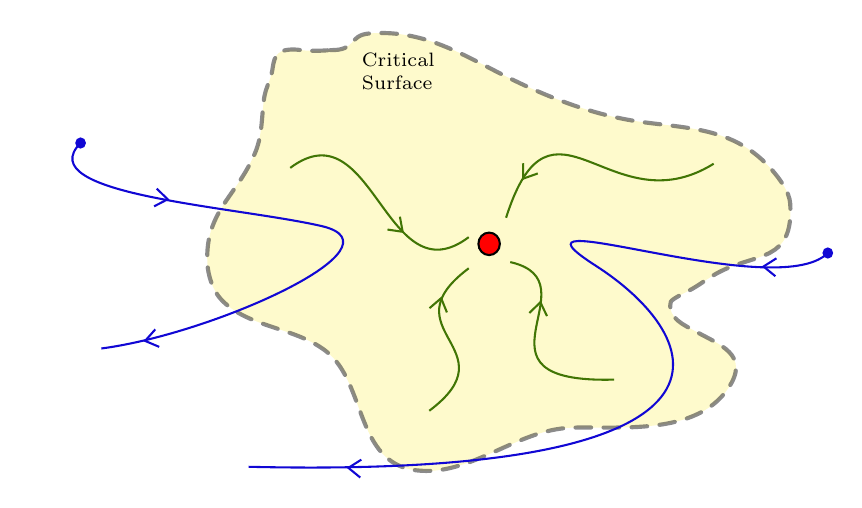
\begin{tikzpicture}[x=0.75pt,y=0.75pt,yscale=-1,xscale=1]
%uncomment if require: \path (0,300); %set diagram left start at 0, and has height of 300

%Curve Lines [id:da7849949621763153] 
\draw [color={rgb, 255:red, 74; green, 74; blue, 74 }  ,draw opacity=0.64 ][fill={rgb, 255:red, 253; green, 242; blue, 133 }  ,fill opacity=0.42 ][line width=1.5] [line join = round][line cap = round] [dash pattern={on 5.63pt off 4.5pt}]  (206.32,43.88) .. controls (219.21,44.16) and (214.87,36.65) .. (225.22,35.85) .. controls (248.43,34.07) and (265.57,43.43) .. (285.33,53.69) .. controls (308.11,65.51) and (331.98,75.35) .. (357.47,78.66) .. controls (381.04,81.72) and (402.12,81.9) .. (419.31,101.85) .. controls (422.66,105.73) and (427.57,112.18) .. (427.9,117.9) .. controls (429.5,146.25) and (412.1,141.26) .. (393.54,150.89) .. controls (389.07,153.22) and (385.04,156.4) .. (380.66,158.92) .. controls (378.85,159.97) and (370.7,163.75) .. (370.36,165.16) .. controls (368.44,173.14) and (377.49,176.66) .. (382.38,179.43) .. controls (393.42,185.69) and (409.22,190.54) .. (397.84,207.08) .. controls (382.08,229.99) and (344.92,224.97) .. (322.26,225.81) .. controls (295.87,226.78) and (273.62,249.57) .. (247.55,246.32) .. controls (218.45,242.69) and (223.5,204.4) .. (204.61,189.24) .. controls (189.75,177.32) and (166.94,177.77) .. (153.94,164.27) .. controls (149.75,159.92) and (147.36,152.58) .. (147.07,146.44) .. controls (145.86,121.29) and (161.59,114.2) .. (170.25,92.93) .. controls (173.76,84.33) and (173.13,75.04) .. (174.55,66.17) .. controls (175.15,62.44) and (177.12,59.06) .. (177.98,55.47) .. controls (179.08,50.93) and (178.49,44.87) .. (184.85,43.88) .. controls (191.93,42.78) and (190.87,45.05) .. (206.32,43.88) -- cycle ;
%Shape: Ellipse [id:dp09682734795909409] 
\draw  [color={rgb, 255:red, 0; green, 0; blue, 0 }  ,draw opacity=1 ][fill={rgb, 255:red, 255; green, 0; blue, 0 }  ,fill opacity=1 ] (277.66,137.21) .. controls (277.66,134.22) and (279.97,131.79) .. (282.83,131.79) .. controls (285.68,131.79) and (288,134.22) .. (288,137.21) .. controls (288,140.21) and (285.68,142.63) .. (282.83,142.63) .. controls (279.97,142.63) and (277.66,140.21) .. (277.66,137.21) -- cycle ;
%Curve Lines [id:da8832046115437673] 
\draw [color={rgb, 255:red, 65; green, 117; blue, 5 }  ,draw opacity=1 ]   (187,100.63) .. controls (227,70.63) and (233,164) .. (273,134) ;
%Curve Lines [id:da948414159458357] 
\draw [color={rgb, 255:red, 65; green, 117; blue, 5 }  ,draw opacity=1 ]   (254,217.63) .. controls (294,187.63) and (233,179) .. (273,149) ;
%Curve Lines [id:da9954148190045367] 
\draw [color={rgb, 255:red, 65; green, 117; blue, 5 }  ,draw opacity=1 ]   (343,202.63) .. controls (267,204.63) and (335,155.63) .. (293,146) ;
%Curve Lines [id:da6038512828805981] 
\draw [color={rgb, 255:red, 65; green, 117; blue, 5 }  ,draw opacity=1 ]   (391,98.63) .. controls (341,129.63) and (313,55.63) .. (291,124.63) ;
%Curve Lines [id:da10801141969503636] 
\draw [color={rgb, 255:red, 17; green, 7; blue, 212 }  ,draw opacity=1 ]   (96,187.63) .. controls (150,180.63) and (244,138.27) .. (202,128.63) .. controls (160,119) and (61,113.63) .. (86,88.63) ;
%Shape: Boxed Bezier Curve [id:dp12977768980803195] 
\draw [color={rgb, 255:red, 17; green, 7; blue, 212 }  ,draw opacity=1 ]   (167,244.63) .. controls (421,250.63) and (387,181.63) .. (334,147.63) .. controls (281,113.63) and (421,166.63) .. (446,141.63) ;
\draw  [color={rgb, 255:red, 17; green, 7; blue, 212 }  ,draw opacity=1 ] (122.67,110.61) -- (127.97,115.76) -- (121.4,119.15) ;
\draw  [color={rgb, 255:red, 17; green, 7; blue, 212 }  ,draw opacity=1 ] (123.88,186.86) -- (117.07,183.98) -- (121.97,178.44) ;
\draw  [color={rgb, 255:red, 17; green, 7; blue, 212 }  ,draw opacity=1 ] (420.74,152.81) -- (415.01,148.14) -- (421.25,144.19) ;
\draw  [color={rgb, 255:red, 17; green, 7; blue, 212 }  ,draw opacity=1 ] (220.74,249.81) -- (215.01,245.14) -- (221.25,241.19) ;
\draw  [color={rgb, 255:red, 65; green, 117; blue, 5 }  ,draw opacity=1 ] (302.22,170.5) -- (307.53,165.36) -- (310.71,172.04) ;
\draw  [color={rgb, 255:red, 65; green, 117; blue, 5 }  ,draw opacity=1 ] (254.1,168.22) -- (259.71,163.4) -- (262.49,170.25) ;
\draw  [color={rgb, 255:red, 65; green, 117; blue, 5 }  ,draw opacity=1 ] (239.84,124.13) -- (241.16,131.4) -- (233.84,130.34) ;
\draw  [color={rgb, 255:red, 65; green, 117; blue, 5 }  ,draw opacity=1 ] (306.26,103.31) -- (299.29,105.78) -- (299.16,98.39) ;
%Shape: Ellipse [id:dp6365405782700908] 
\draw  [draw opacity=0][fill={rgb, 255:red, 17; green, 7; blue, 212 }  ,fill opacity=1 ] (83.41,88.63) .. controls (83.41,87.14) and (84.57,85.92) .. (86,85.92) .. controls (87.43,85.92) and (88.59,87.14) .. (88.59,88.63) .. controls (88.59,90.13) and (87.43,91.34) .. (86,91.34) .. controls (84.57,91.34) and (83.41,90.13) .. (83.41,88.63) -- cycle ;
%Shape: Ellipse [id:dp26949101542259046] 
\draw  [draw opacity=0][fill={rgb, 255:red, 17; green, 7; blue, 212 }  ,fill opacity=1 ] (443.41,141.63) .. controls (443.41,140.14) and (444.57,138.92) .. (446,138.92) .. controls (447.43,138.92) and (448.59,140.14) .. (448.59,141.63) .. controls (448.59,143.13) and (447.43,144.34) .. (446,144.34) .. controls (444.57,144.34) and (443.41,143.13) .. (443.41,141.63) -- cycle ;

% Text Node
\draw (220,44) node [anchor=north west][inner sep=0.75pt]  [font=\scriptsize] [align=left] {Critical \\Surface};


\end{tikzpicture}

    \caption{\textbf{RG flow in K-space.} The blue arrows denote the relevant flows, outside of the critical surface while the green arrows show the irrelevant flows towards the fixed point (red marker), on the critical surface. The critical surface is denoted by the yellow region.}
\end{figure}

\subsection{RG for 2D Ising Model on square lattice}
Let us see RG in play for the zero-field 2D Ising model, whose Hamiltonian is given by 
\begin{align}\label{ising2dham}
    -\beta \SH = K \sum\limits_{\avg{ij}} \sigma_i \sigma_j
\end{align}
where $K=\beta J$. Then the partition function becomes,
$$\SZ = \sum\limits_{\{\sigma_k\}} \exp\qty[K \sum\limits_{\avg{ij}} \sigma_i \sigma_j] = \sum\limits_{\{\sigma_k\}}\prod\limits_{\avg{ij}} \exp\qty[K  \sigma_i \sigma_j]$$
As before, let us take a particular spin, say $\sigma_{(i,j)}$ (where $(i,j)$ represents the coordinate on the lattice), and then trace it out. The term $\sigma_{(i,j)}$ appears in: 
\begin{align*}
    \SZ_N &=\qty{\sum\limits_{\substack{\sigma_{p\neq i,\, q\neq j}\\ = \pm 1}}} \sum\limits_{\substack{\sigma_{(i,j)}\\ = \pm 1}}\cdots \exp\qty[K\sigma_{(i,j-1)}\sigma_{(i,j)}]\cdot\exp\qty[K\sigma_{(i,j+1)}\sigma_{(i,j)}]\cdot\exp\qty[K\sigma_{(i,j)}\sigma_{(i-1,j)}]\cdot\exp\qty[K\sigma_{(i,j)}\sigma_{(i+1,j)}]\cdots\\
&=\sum\limits_{\sigma_{p\neq i, q\neq j}= \pm 1}\cdots \cdot\qty[2\cosh \qty(K(\sigma_{(i,j+1)}+\sigma_{(i,j-1)}+\sigma_{(i+1,j)}+\sigma_{(i-1,j)}))]\cdots
\end{align*}
\begin{figure}[t]
    \centering 
    

\tikzset{every picture/.style={line width=0.75pt}} %set default line width to 0.75pt        

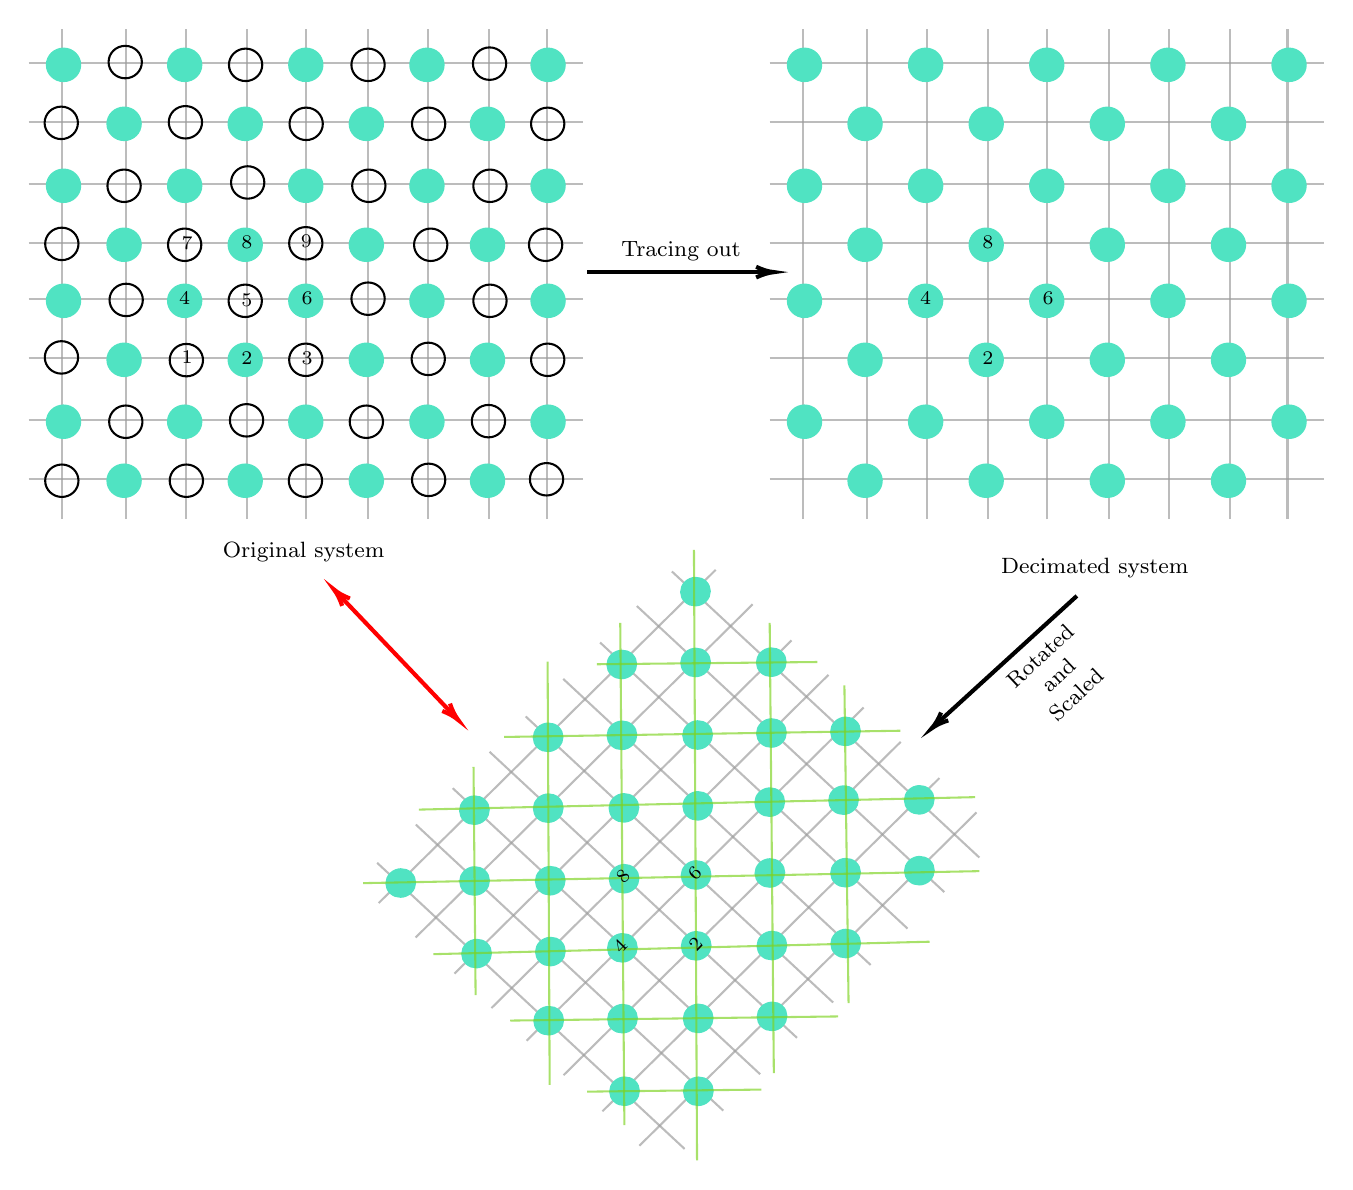
\begin{tikzpicture}[x=0.75pt,y=0.75pt,yscale=-1,xscale=1]
%uncomment if require: \path (0,574); %set diagram left start at 0, and has height of 574

%Straight Lines [id:da43774284862597024] 
\draw [color={rgb, 255:red, 155; green, 155; blue, 155 }  ,draw opacity=0.67 ]   (125.05,260.48) -- (125.05,24.25) ;
%Straight Lines [id:da6936548161724166] 
\draw [color={rgb, 255:red, 155; green, 155; blue, 155 }  ,draw opacity=0.67 ]   (153.5,260.65) -- (153.5,24.41) ;
%Straight Lines [id:da43250215442689033] 
\draw [color={rgb, 255:red, 155; green, 155; blue, 155 }  ,draw opacity=0.67 ]   (183.41,260.48) -- (183.41,24.25) ;
%Straight Lines [id:da02433371577239829] 
\draw [color={rgb, 255:red, 155; green, 155; blue, 155 }  ,draw opacity=0.67 ]   (212.59,260.48) -- (212.59,24.25) ;
%Straight Lines [id:da6103239717866829] 
\draw [color={rgb, 255:red, 155; green, 155; blue, 155 }  ,draw opacity=0.67 ]   (241.77,260.48) -- (241.77,24.25) ;
%Straight Lines [id:da5949120872771251] 
\draw [color={rgb, 255:red, 155; green, 155; blue, 155 }  ,draw opacity=0.67 ]   (269.49,260.48) -- (269.49,24.25) ;
%Straight Lines [id:da41162656601198744] 
\draw [color={rgb, 255:red, 155; green, 155; blue, 155 }  ,draw opacity=0.67 ]   (36.05,260.48) -- (36.05,24.25) ;
%Straight Lines [id:da17761311427248883] 
\draw [color={rgb, 255:red, 155; green, 155; blue, 155 }  ,draw opacity=0.67 ]   (66.69,260.48) -- (66.69,24.25) ;
%Straight Lines [id:da6566420944033906] 
\draw [color={rgb, 255:red, 155; green, 155; blue, 155 }  ,draw opacity=0.67 ]   (95.87,260.48) -- (95.87,24.25) ;
%Straight Lines [id:da524390367375496] 
\draw [color={rgb, 255:red, 155; green, 155; blue, 155 }  ,draw opacity=0.67 ]   (20,40.95) -- (287,40.95) ;
%Shape: Ellipse [id:dp14367798514224728] 
\draw  [color={rgb, 255:red, 80; green, 227; blue, 194 }  ,draw opacity=1 ][fill={rgb, 255:red, 80; green, 227; blue, 194 }  ,fill opacity=1 ] (28.75,41.66) .. controls (28.75,37.34) and (32.35,33.84) .. (36.78,33.84) .. controls (41.21,33.84) and (44.8,37.34) .. (44.8,41.66) .. controls (44.8,45.98) and (41.21,49.47) .. (36.78,49.47) .. controls (32.35,49.47) and (28.75,45.98) .. (28.75,41.66) -- cycle ;
%Shape: Ellipse [id:dp3599045556083088] 
\draw  [color={rgb, 255:red, 80; green, 227; blue, 194 }  ,draw opacity=1 ][fill={rgb, 255:red, 80; green, 227; blue, 194 }  ,fill opacity=1 ] (87.11,41.66) .. controls (87.11,37.34) and (90.71,33.84) .. (95.14,33.84) .. controls (99.57,33.84) and (103.16,37.34) .. (103.16,41.66) .. controls (103.16,45.98) and (99.57,49.47) .. (95.14,49.47) .. controls (90.71,49.47) and (87.11,45.98) .. (87.11,41.66) -- cycle ;
%Shape: Ellipse [id:dp3995051616717167] 
\draw  [color={rgb, 255:red, 80; green, 227; blue, 194 }  ,draw opacity=1 ][fill={rgb, 255:red, 80; green, 227; blue, 194 }  ,fill opacity=1 ] (145.48,41.66) .. controls (145.48,37.34) and (149.07,33.84) .. (153.5,33.84) .. controls (157.93,33.84) and (161.52,37.34) .. (161.52,41.66) .. controls (161.52,45.98) and (157.93,49.47) .. (153.5,49.47) .. controls (149.07,49.47) and (145.48,45.98) .. (145.48,41.66) -- cycle ;
%Shape: Ellipse [id:dp3109774679588371] 
\draw  [color={rgb, 255:red, 80; green, 227; blue, 194 }  ,draw opacity=1 ][fill={rgb, 255:red, 80; green, 227; blue, 194 }  ,fill opacity=1 ] (203.84,41.66) .. controls (203.84,37.34) and (207.43,33.84) .. (211.86,33.84) .. controls (216.29,33.84) and (219.89,37.34) .. (219.89,41.66) .. controls (219.89,45.98) and (216.29,49.47) .. (211.86,49.47) .. controls (207.43,49.47) and (203.84,45.98) .. (203.84,41.66) -- cycle ;
%Shape: Ellipse [id:dp8032998539588463] 
\draw  [color={rgb, 255:red, 80; green, 227; blue, 194 }  ,draw opacity=1 ][fill={rgb, 255:red, 80; green, 227; blue, 194 }  ,fill opacity=1 ] (262.2,41.66) .. controls (262.2,37.34) and (265.79,33.84) .. (270.22,33.84) .. controls (274.65,33.84) and (278.25,37.34) .. (278.25,41.66) .. controls (278.25,45.98) and (274.65,49.47) .. (270.22,49.47) .. controls (265.79,49.47) and (262.2,45.98) .. (262.2,41.66) -- cycle ;
%Straight Lines [id:da017718299737276344] 
\draw [color={rgb, 255:red, 155; green, 155; blue, 155 }  ,draw opacity=0.67 ]   (20,69.37) -- (287,69.37) ;
%Shape: Ellipse [id:dp747306266103335] 
\draw  [color={rgb, 255:red, 80; green, 227; blue, 194 }  ,draw opacity=1 ][fill={rgb, 255:red, 80; green, 227; blue, 194 }  ,fill opacity=1 ] (57.93,70.08) .. controls (57.93,65.76) and (61.53,62.26) .. (65.96,62.26) .. controls (70.39,62.26) and (73.98,65.76) .. (73.98,70.08) .. controls (73.98,74.4) and (70.39,77.9) .. (65.96,77.9) .. controls (61.53,77.9) and (57.93,74.4) .. (57.93,70.08) -- cycle ;
%Shape: Ellipse [id:dp7852324690422746] 
\draw  [color={rgb, 255:red, 80; green, 227; blue, 194 }  ,draw opacity=1 ][fill={rgb, 255:red, 80; green, 227; blue, 194 }  ,fill opacity=1 ] (116.3,70.08) .. controls (116.3,65.76) and (119.89,62.26) .. (124.32,62.26) .. controls (128.75,62.26) and (132.34,65.76) .. (132.34,70.08) .. controls (132.34,74.4) and (128.75,77.9) .. (124.32,77.9) .. controls (119.89,77.9) and (116.3,74.4) .. (116.3,70.08) -- cycle ;
%Shape: Ellipse [id:dp6080600416519873] 
\draw  [color={rgb, 255:red, 80; green, 227; blue, 194 }  ,draw opacity=1 ][fill={rgb, 255:red, 80; green, 227; blue, 194 }  ,fill opacity=1 ] (174.66,70.08) .. controls (174.66,65.76) and (178.25,62.26) .. (182.68,62.26) .. controls (187.11,62.26) and (190.7,65.76) .. (190.7,70.08) .. controls (190.7,74.4) and (187.11,77.9) .. (182.68,77.9) .. controls (178.25,77.9) and (174.66,74.4) .. (174.66,70.08) -- cycle ;
%Shape: Ellipse [id:dp7924435754339052] 
\draw  [color={rgb, 255:red, 80; green, 227; blue, 194 }  ,draw opacity=1 ][fill={rgb, 255:red, 80; green, 227; blue, 194 }  ,fill opacity=1 ] (233.02,70.08) .. controls (233.02,65.76) and (236.61,62.26) .. (241.04,62.26) .. controls (245.47,62.26) and (249.07,65.76) .. (249.07,70.08) .. controls (249.07,74.4) and (245.47,77.9) .. (241.04,77.9) .. controls (236.61,77.9) and (233.02,74.4) .. (233.02,70.08) -- cycle ;
%Straight Lines [id:da3600072332140696] 
\draw [color={rgb, 255:red, 155; green, 155; blue, 155 }  ,draw opacity=0.67 ]   (20,99.21) -- (287,99.21) ;
%Shape: Ellipse [id:dp3964139277090135] 
\draw  [color={rgb, 255:red, 80; green, 227; blue, 194 }  ,draw opacity=1 ][fill={rgb, 255:red, 80; green, 227; blue, 194 }  ,fill opacity=1 ] (28.75,99.92) .. controls (28.75,95.61) and (32.35,92.11) .. (36.78,92.11) .. controls (41.21,92.11) and (44.8,95.61) .. (44.8,99.92) .. controls (44.8,104.24) and (41.21,107.74) .. (36.78,107.74) .. controls (32.35,107.74) and (28.75,104.24) .. (28.75,99.92) -- cycle ;
%Shape: Ellipse [id:dp8782123955194711] 
\draw  [color={rgb, 255:red, 0; green, 0; blue, 0 }  ,draw opacity=1 ] (57.93,99.92) .. controls (57.93,95.61) and (61.53,92.11) .. (65.96,92.11) .. controls (70.39,92.11) and (73.98,95.61) .. (73.98,99.92) .. controls (73.98,104.24) and (70.39,107.74) .. (65.96,107.74) .. controls (61.53,107.74) and (57.93,104.24) .. (57.93,99.92) -- cycle ;
%Shape: Ellipse [id:dp18480339323298367] 
\draw  [color={rgb, 255:red, 80; green, 227; blue, 194 }  ,draw opacity=1 ][fill={rgb, 255:red, 80; green, 227; blue, 194 }  ,fill opacity=1 ] (87.11,99.92) .. controls (87.11,95.61) and (90.71,92.11) .. (95.14,92.11) .. controls (99.57,92.11) and (103.16,95.61) .. (103.16,99.92) .. controls (103.16,104.24) and (99.57,107.74) .. (95.14,107.74) .. controls (90.71,107.74) and (87.11,104.24) .. (87.11,99.92) -- cycle ;
%Shape: Ellipse [id:dp4424147155896917] 
\draw  [color={rgb, 255:red, 80; green, 227; blue, 194 }  ,draw opacity=1 ][fill={rgb, 255:red, 80; green, 227; blue, 194 }  ,fill opacity=1 ] (145.48,99.92) .. controls (145.48,95.61) and (149.07,92.11) .. (153.5,92.11) .. controls (157.93,92.11) and (161.52,95.61) .. (161.52,99.92) .. controls (161.52,104.24) and (157.93,107.74) .. (153.5,107.74) .. controls (149.07,107.74) and (145.48,104.24) .. (145.48,99.92) -- cycle ;
%Shape: Ellipse [id:dp6808213664790959] 
\draw  [color={rgb, 255:red, 80; green, 227; blue, 194 }  ,draw opacity=1 ][fill={rgb, 255:red, 80; green, 227; blue, 194 }  ,fill opacity=1 ] (203.84,99.92) .. controls (203.84,95.61) and (207.43,92.11) .. (211.86,92.11) .. controls (216.29,92.11) and (219.89,95.61) .. (219.89,99.92) .. controls (219.89,104.24) and (216.29,107.74) .. (211.86,107.74) .. controls (207.43,107.74) and (203.84,104.24) .. (203.84,99.92) -- cycle ;
%Shape: Ellipse [id:dp06283383505588935] 
\draw  [color={rgb, 255:red, 80; green, 227; blue, 194 }  ,draw opacity=1 ][fill={rgb, 255:red, 80; green, 227; blue, 194 }  ,fill opacity=1 ] (262.2,99.92) .. controls (262.2,95.61) and (265.79,92.11) .. (270.22,92.11) .. controls (274.65,92.11) and (278.25,95.61) .. (278.25,99.92) .. controls (278.25,104.24) and (274.65,107.74) .. (270.22,107.74) .. controls (265.79,107.74) and (262.2,104.24) .. (262.2,99.92) -- cycle ;
%Straight Lines [id:da18214636407385543] 
\draw [color={rgb, 255:red, 155; green, 155; blue, 155 }  ,draw opacity=0.67 ]   (20,127.63) -- (287,127.63) ;
%Shape: Ellipse [id:dp07825821892535378] 
\draw  [color={rgb, 255:red, 80; green, 227; blue, 194 }  ,draw opacity=1 ][fill={rgb, 255:red, 80; green, 227; blue, 194 }  ,fill opacity=1 ] (57.93,128.35) .. controls (57.93,124.03) and (61.53,120.53) .. (65.96,120.53) .. controls (70.39,120.53) and (73.98,124.03) .. (73.98,128.35) .. controls (73.98,132.66) and (70.39,136.16) .. (65.96,136.16) .. controls (61.53,136.16) and (57.93,132.66) .. (57.93,128.35) -- cycle ;
%Shape: Ellipse [id:dp1066084129479733] 
\draw  [color={rgb, 255:red, 0; green, 0; blue, 0 }  ,draw opacity=1 ] (87.11,128.35) .. controls (87.11,124.03) and (90.71,120.53) .. (95.14,120.53) .. controls (99.57,120.53) and (103.16,124.03) .. (103.16,128.35) .. controls (103.16,132.66) and (99.57,136.16) .. (95.14,136.16) .. controls (90.71,136.16) and (87.11,132.66) .. (87.11,128.35) -- cycle ;
%Shape: Ellipse [id:dp560948579160624] 
\draw  [color={rgb, 255:red, 80; green, 227; blue, 194 }  ,draw opacity=1 ][fill={rgb, 255:red, 80; green, 227; blue, 194 }  ,fill opacity=1 ] (116.3,128.35) .. controls (116.3,124.03) and (119.89,120.53) .. (124.32,120.53) .. controls (128.75,120.53) and (132.34,124.03) .. (132.34,128.35) .. controls (132.34,132.66) and (128.75,136.16) .. (124.32,136.16) .. controls (119.89,136.16) and (116.3,132.66) .. (116.3,128.35) -- cycle ;
%Shape: Ellipse [id:dp2940882042723849] 
\draw  [color={rgb, 255:red, 80; green, 227; blue, 194 }  ,draw opacity=1 ][fill={rgb, 255:red, 80; green, 227; blue, 194 }  ,fill opacity=1 ] (174.66,128.35) .. controls (174.66,124.03) and (178.25,120.53) .. (182.68,120.53) .. controls (187.11,120.53) and (190.7,124.03) .. (190.7,128.35) .. controls (190.7,132.66) and (187.11,136.16) .. (182.68,136.16) .. controls (178.25,136.16) and (174.66,132.66) .. (174.66,128.35) -- cycle ;
%Shape: Ellipse [id:dp14003035278586162] 
\draw  [color={rgb, 255:red, 80; green, 227; blue, 194 }  ,draw opacity=1 ][fill={rgb, 255:red, 80; green, 227; blue, 194 }  ,fill opacity=1 ] (233.02,128.35) .. controls (233.02,124.03) and (236.61,120.53) .. (241.04,120.53) .. controls (245.47,120.53) and (249.07,124.03) .. (249.07,128.35) .. controls (249.07,132.66) and (245.47,136.16) .. (241.04,136.16) .. controls (236.61,136.16) and (233.02,132.66) .. (233.02,128.35) -- cycle ;
%Straight Lines [id:da24325373078178347] 
\draw [color={rgb, 255:red, 155; green, 155; blue, 155 }  ,draw opacity=0.67 ]   (20,154.64) -- (287,154.64) ;
%Shape: Ellipse [id:dp8555722072410666] 
\draw  [color={rgb, 255:red, 80; green, 227; blue, 194 }  ,draw opacity=1 ][fill={rgb, 255:red, 80; green, 227; blue, 194 }  ,fill opacity=1 ] (28.75,155.35) .. controls (28.75,151.03) and (32.35,147.53) .. (36.78,147.53) .. controls (41.21,147.53) and (44.8,151.03) .. (44.8,155.35) .. controls (44.8,159.66) and (41.21,163.16) .. (36.78,163.16) .. controls (32.35,163.16) and (28.75,159.66) .. (28.75,155.35) -- cycle ;
%Shape: Ellipse [id:dp5486111221116741] 
\draw  [color={rgb, 255:red, 80; green, 227; blue, 194 }  ,draw opacity=1 ][fill={rgb, 255:red, 80; green, 227; blue, 194 }  ,fill opacity=1 ] (87.11,155.35) .. controls (87.11,151.03) and (90.71,147.53) .. (95.14,147.53) .. controls (99.57,147.53) and (103.16,151.03) .. (103.16,155.35) .. controls (103.16,159.66) and (99.57,163.16) .. (95.14,163.16) .. controls (90.71,163.16) and (87.11,159.66) .. (87.11,155.35) -- cycle ;
%Shape: Ellipse [id:dp9510498910971997] 
\draw  [color={rgb, 255:red, 0; green, 0; blue, 0 }  ,draw opacity=1 ] (116.3,155.35) .. controls (116.3,151.03) and (119.89,147.53) .. (124.32,147.53) .. controls (128.75,147.53) and (132.34,151.03) .. (132.34,155.35) .. controls (132.34,159.66) and (128.75,163.16) .. (124.32,163.16) .. controls (119.89,163.16) and (116.3,159.66) .. (116.3,155.35) -- cycle ;
%Shape: Ellipse [id:dp09185871433127435] 
\draw  [color={rgb, 255:red, 80; green, 227; blue, 194 }  ,draw opacity=1 ][fill={rgb, 255:red, 80; green, 227; blue, 194 }  ,fill opacity=1 ] (145.48,155.35) .. controls (145.48,151.03) and (149.07,147.53) .. (153.5,147.53) .. controls (157.93,147.53) and (161.52,151.03) .. (161.52,155.35) .. controls (161.52,159.66) and (157.93,163.16) .. (153.5,163.16) .. controls (149.07,163.16) and (145.48,159.66) .. (145.48,155.35) -- cycle ;
%Shape: Ellipse [id:dp5499602017761521] 
\draw  [color={rgb, 255:red, 80; green, 227; blue, 194 }  ,draw opacity=1 ][fill={rgb, 255:red, 80; green, 227; blue, 194 }  ,fill opacity=1 ] (203.84,155.35) .. controls (203.84,151.03) and (207.43,147.53) .. (211.86,147.53) .. controls (216.29,147.53) and (219.89,151.03) .. (219.89,155.35) .. controls (219.89,159.66) and (216.29,163.16) .. (211.86,163.16) .. controls (207.43,163.16) and (203.84,159.66) .. (203.84,155.35) -- cycle ;
%Shape: Ellipse [id:dp2639410840908075] 
\draw  [color={rgb, 255:red, 80; green, 227; blue, 194 }  ,draw opacity=1 ][fill={rgb, 255:red, 80; green, 227; blue, 194 }  ,fill opacity=1 ] (262.2,155.35) .. controls (262.2,151.03) and (265.79,147.53) .. (270.22,147.53) .. controls (274.65,147.53) and (278.25,151.03) .. (278.25,155.35) .. controls (278.25,159.66) and (274.65,163.16) .. (270.22,163.16) .. controls (265.79,163.16) and (262.2,159.66) .. (262.2,155.35) -- cycle ;
%Straight Lines [id:da32485767615916683] 
\draw [color={rgb, 255:red, 155; green, 155; blue, 155 }  ,draw opacity=0.67 ]   (20,183.06) -- (287,183.06) ;
%Shape: Ellipse [id:dp33550256997370786] 
\draw  [color={rgb, 255:red, 80; green, 227; blue, 194 }  ,draw opacity=1 ][fill={rgb, 255:red, 80; green, 227; blue, 194 }  ,fill opacity=1 ] (57.93,183.77) .. controls (57.93,179.45) and (61.53,175.95) .. (65.96,175.95) .. controls (70.39,175.95) and (73.98,179.45) .. (73.98,183.77) .. controls (73.98,188.08) and (70.39,191.58) .. (65.96,191.58) .. controls (61.53,191.58) and (57.93,188.08) .. (57.93,183.77) -- cycle ;
%Shape: Ellipse [id:dp4539953612932256] 
\draw  [color={rgb, 255:red, 80; green, 227; blue, 194 }  ,draw opacity=1 ][fill={rgb, 255:red, 80; green, 227; blue, 194 }  ,fill opacity=1 ] (116.3,183.77) .. controls (116.3,179.45) and (119.89,175.95) .. (124.32,175.95) .. controls (128.75,175.95) and (132.34,179.45) .. (132.34,183.77) .. controls (132.34,188.08) and (128.75,191.58) .. (124.32,191.58) .. controls (119.89,191.58) and (116.3,188.08) .. (116.3,183.77) -- cycle ;
%Shape: Ellipse [id:dp5515753241900382] 
\draw  [color={rgb, 255:red, 0; green, 0; blue, 0 }  ,draw opacity=1 ] (145.48,183.77) .. controls (145.48,179.45) and (149.07,175.95) .. (153.5,175.95) .. controls (157.93,175.95) and (161.52,179.45) .. (161.52,183.77) .. controls (161.52,188.08) and (157.93,191.58) .. (153.5,191.58) .. controls (149.07,191.58) and (145.48,188.08) .. (145.48,183.77) -- cycle ;
%Shape: Ellipse [id:dp966221615897664] 
\draw  [color={rgb, 255:red, 80; green, 227; blue, 194 }  ,draw opacity=1 ][fill={rgb, 255:red, 80; green, 227; blue, 194 }  ,fill opacity=1 ] (174.66,183.77) .. controls (174.66,179.45) and (178.25,175.95) .. (182.68,175.95) .. controls (187.11,175.95) and (190.7,179.45) .. (190.7,183.77) .. controls (190.7,188.08) and (187.11,191.58) .. (182.68,191.58) .. controls (178.25,191.58) and (174.66,188.08) .. (174.66,183.77) -- cycle ;
%Shape: Ellipse [id:dp7878977235745577] 
\draw  [color={rgb, 255:red, 80; green, 227; blue, 194 }  ,draw opacity=1 ][fill={rgb, 255:red, 80; green, 227; blue, 194 }  ,fill opacity=1 ] (233.02,183.77) .. controls (233.02,179.45) and (236.61,175.95) .. (241.04,175.95) .. controls (245.47,175.95) and (249.07,179.45) .. (249.07,183.77) .. controls (249.07,188.08) and (245.47,191.58) .. (241.04,191.58) .. controls (236.61,191.58) and (233.02,188.08) .. (233.02,183.77) -- cycle ;
%Straight Lines [id:da8780890851287075] 
\draw [color={rgb, 255:red, 155; green, 155; blue, 155 }  ,draw opacity=0.67 ]   (20,212.9) -- (287,212.9) ;
%Shape: Ellipse [id:dp06469123213132943] 
\draw  [color={rgb, 255:red, 80; green, 227; blue, 194 }  ,draw opacity=1 ][fill={rgb, 255:red, 80; green, 227; blue, 194 }  ,fill opacity=1 ] (28.75,213.61) .. controls (28.75,209.29) and (32.35,205.79) .. (36.78,205.79) .. controls (41.21,205.79) and (44.8,209.29) .. (44.8,213.61) .. controls (44.8,217.93) and (41.21,221.43) .. (36.78,221.43) .. controls (32.35,221.43) and (28.75,217.93) .. (28.75,213.61) -- cycle ;
%Shape: Ellipse [id:dp5930386669148578] 
\draw  [color={rgb, 255:red, 80; green, 227; blue, 194 }  ,draw opacity=1 ][fill={rgb, 255:red, 80; green, 227; blue, 194 }  ,fill opacity=1 ] (87.11,213.61) .. controls (87.11,209.29) and (90.71,205.79) .. (95.14,205.79) .. controls (99.57,205.79) and (103.16,209.29) .. (103.16,213.61) .. controls (103.16,217.93) and (99.57,221.43) .. (95.14,221.43) .. controls (90.71,221.43) and (87.11,217.93) .. (87.11,213.61) -- cycle ;
%Shape: Ellipse [id:dp9997599283957436] 
\draw  [color={rgb, 255:red, 80; green, 227; blue, 194 }  ,draw opacity=1 ][fill={rgb, 255:red, 80; green, 227; blue, 194 }  ,fill opacity=1 ] (145.48,213.61) .. controls (145.48,209.29) and (149.07,205.79) .. (153.5,205.79) .. controls (157.93,205.79) and (161.52,209.29) .. (161.52,213.61) .. controls (161.52,217.93) and (157.93,221.43) .. (153.5,221.43) .. controls (149.07,221.43) and (145.48,217.93) .. (145.48,213.61) -- cycle ;
%Shape: Ellipse [id:dp8094865622076323] 
\draw  [color={rgb, 255:red, 0; green, 0; blue, 0 }  ,draw opacity=1 ] (174.66,213.61) .. controls (174.66,209.29) and (178.25,205.79) .. (182.68,205.79) .. controls (187.11,205.79) and (190.7,209.29) .. (190.7,213.61) .. controls (190.7,217.93) and (187.11,221.43) .. (182.68,221.43) .. controls (178.25,221.43) and (174.66,217.93) .. (174.66,213.61) -- cycle ;
%Shape: Ellipse [id:dp19624336417026012] 
\draw  [color={rgb, 255:red, 80; green, 227; blue, 194 }  ,draw opacity=1 ][fill={rgb, 255:red, 80; green, 227; blue, 194 }  ,fill opacity=1 ] (203.84,213.61) .. controls (203.84,209.29) and (207.43,205.79) .. (211.86,205.79) .. controls (216.29,205.79) and (219.89,209.29) .. (219.89,213.61) .. controls (219.89,217.93) and (216.29,221.43) .. (211.86,221.43) .. controls (207.43,221.43) and (203.84,217.93) .. (203.84,213.61) -- cycle ;
%Shape: Ellipse [id:dp48744496868814113] 
\draw  [color={rgb, 255:red, 80; green, 227; blue, 194 }  ,draw opacity=1 ][fill={rgb, 255:red, 80; green, 227; blue, 194 }  ,fill opacity=1 ] (262.2,213.61) .. controls (262.2,209.29) and (265.79,205.79) .. (270.22,205.79) .. controls (274.65,205.79) and (278.25,209.29) .. (278.25,213.61) .. controls (278.25,217.93) and (274.65,221.43) .. (270.22,221.43) .. controls (265.79,221.43) and (262.2,217.93) .. (262.2,213.61) -- cycle ;
%Straight Lines [id:da7578668340854509] 
\draw [color={rgb, 255:red, 155; green, 155; blue, 155 }  ,draw opacity=0.67 ]   (20,241.32) -- (287,241.32) ;
%Shape: Ellipse [id:dp12742050580735043] 
\draw  [color={rgb, 255:red, 80; green, 227; blue, 194 }  ,draw opacity=1 ][fill={rgb, 255:red, 80; green, 227; blue, 194 }  ,fill opacity=1 ] (57.93,242.03) .. controls (57.93,237.72) and (61.53,234.22) .. (65.96,234.22) .. controls (70.39,234.22) and (73.98,237.72) .. (73.98,242.03) .. controls (73.98,246.35) and (70.39,249.85) .. (65.96,249.85) .. controls (61.53,249.85) and (57.93,246.35) .. (57.93,242.03) -- cycle ;
%Shape: Ellipse [id:dp7335998318232068] 
\draw  [color={rgb, 255:red, 80; green, 227; blue, 194 }  ,draw opacity=1 ][fill={rgb, 255:red, 80; green, 227; blue, 194 }  ,fill opacity=1 ] (116.3,242.03) .. controls (116.3,237.72) and (119.89,234.22) .. (124.32,234.22) .. controls (128.75,234.22) and (132.34,237.72) .. (132.34,242.03) .. controls (132.34,246.35) and (128.75,249.85) .. (124.32,249.85) .. controls (119.89,249.85) and (116.3,246.35) .. (116.3,242.03) -- cycle ;
%Shape: Ellipse [id:dp2410303674058174] 
\draw  [color={rgb, 255:red, 80; green, 227; blue, 194 }  ,draw opacity=1 ][fill={rgb, 255:red, 80; green, 227; blue, 194 }  ,fill opacity=1 ] (174.66,242.03) .. controls (174.66,237.72) and (178.25,234.22) .. (182.68,234.22) .. controls (187.11,234.22) and (190.7,237.72) .. (190.7,242.03) .. controls (190.7,246.35) and (187.11,249.85) .. (182.68,249.85) .. controls (178.25,249.85) and (174.66,246.35) .. (174.66,242.03) -- cycle ;
%Shape: Ellipse [id:dp9092422841555949] 
\draw  [color={rgb, 255:red, 80; green, 227; blue, 194 }  ,draw opacity=1 ][fill={rgb, 255:red, 80; green, 227; blue, 194 }  ,fill opacity=1 ] (233.02,242.03) .. controls (233.02,237.72) and (236.61,234.22) .. (241.04,234.22) .. controls (245.47,234.22) and (249.07,237.72) .. (249.07,242.03) .. controls (249.07,246.35) and (245.47,249.85) .. (241.04,249.85) .. controls (236.61,249.85) and (233.02,246.35) .. (233.02,242.03) -- cycle ;
%Shape: Ellipse [id:dp6302085329803937] 
\draw  [color={rgb, 255:red, 0; green, 0; blue, 0 }  ,draw opacity=1 ] (204.66,241.61) .. controls (204.66,237.29) and (208.25,233.79) .. (212.68,233.79) .. controls (217.11,233.79) and (220.7,237.29) .. (220.7,241.61) .. controls (220.7,245.93) and (217.11,249.43) .. (212.68,249.43) .. controls (208.25,249.43) and (204.66,245.93) .. (204.66,241.61) -- cycle ;
%Shape: Ellipse [id:dp18968588855728563] 
\draw  [color={rgb, 255:red, 0; green, 0; blue, 0 }  ,draw opacity=1 ] (27.66,69.61) .. controls (27.66,65.29) and (31.25,61.79) .. (35.68,61.79) .. controls (40.11,61.79) and (43.7,65.29) .. (43.7,69.61) .. controls (43.7,73.93) and (40.11,77.43) .. (35.68,77.43) .. controls (31.25,77.43) and (27.66,73.93) .. (27.66,69.61) -- cycle ;
%Shape: Ellipse [id:dp113136754455754] 
\draw  [color={rgb, 255:red, 0; green, 0; blue, 0 }  ,draw opacity=1 ] (27.93,127.92) .. controls (27.93,123.61) and (31.53,120.11) .. (35.96,120.11) .. controls (40.39,120.11) and (43.98,123.61) .. (43.98,127.92) .. controls (43.98,132.24) and (40.39,135.74) .. (35.96,135.74) .. controls (31.53,135.74) and (27.93,132.24) .. (27.93,127.92) -- cycle ;
%Shape: Ellipse [id:dp771965243992261] 
\draw  [color={rgb, 255:red, 0; green, 0; blue, 0 }  ,draw opacity=1 ] (58.93,154.92) .. controls (58.93,150.61) and (62.53,147.11) .. (66.96,147.11) .. controls (71.39,147.11) and (74.98,150.61) .. (74.98,154.92) .. controls (74.98,159.24) and (71.39,162.74) .. (66.96,162.74) .. controls (62.53,162.74) and (58.93,159.24) .. (58.93,154.92) -- cycle ;
%Shape: Ellipse [id:dp7386213349134408] 
\draw  [color={rgb, 255:red, 0; green, 0; blue, 0 }  ,draw opacity=1 ] (87.93,183.92) .. controls (87.93,179.61) and (91.53,176.11) .. (95.96,176.11) .. controls (100.39,176.11) and (103.98,179.61) .. (103.98,183.92) .. controls (103.98,188.24) and (100.39,191.74) .. (95.96,191.74) .. controls (91.53,191.74) and (87.93,188.24) .. (87.93,183.92) -- cycle ;
%Shape: Ellipse [id:dp5713443485000416] 
\draw  [color={rgb, 255:red, 0; green, 0; blue, 0 }  ,draw opacity=1 ] (116.93,212.92) .. controls (116.93,208.61) and (120.53,205.11) .. (124.96,205.11) .. controls (129.39,205.11) and (132.98,208.61) .. (132.98,212.92) .. controls (132.98,217.24) and (129.39,220.74) .. (124.96,220.74) .. controls (120.53,220.74) and (116.93,217.24) .. (116.93,212.92) -- cycle ;
%Shape: Ellipse [id:dp2363386078273908] 
\draw  [color={rgb, 255:red, 0; green, 0; blue, 0 }  ,draw opacity=1 ] (233.48,213.32) .. controls (233.48,209.01) and (237.07,205.51) .. (241.5,205.51) .. controls (245.93,205.51) and (249.52,209.01) .. (249.52,213.32) .. controls (249.52,217.64) and (245.93,221.14) .. (241.5,221.14) .. controls (237.07,221.14) and (233.48,217.64) .. (233.48,213.32) -- cycle ;
%Shape: Ellipse [id:dp40382143925142433] 
\draw  [color={rgb, 255:red, 0; green, 0; blue, 0 }  ,draw opacity=1 ] (145.3,242.03) .. controls (145.3,237.72) and (148.89,234.22) .. (153.32,234.22) .. controls (157.75,234.22) and (161.34,237.72) .. (161.34,242.03) .. controls (161.34,246.35) and (157.75,249.85) .. (153.32,249.85) .. controls (148.89,249.85) and (145.3,246.35) .. (145.3,242.03) -- cycle ;
%Shape: Ellipse [id:dp7113892107991495] 
\draw  [color={rgb, 255:red, 0; green, 0; blue, 0 }  ,draw opacity=1 ] (204.48,183.32) .. controls (204.48,179.01) and (208.07,175.51) .. (212.5,175.51) .. controls (216.93,175.51) and (220.52,179.01) .. (220.52,183.32) .. controls (220.52,187.64) and (216.93,191.14) .. (212.5,191.14) .. controls (208.07,191.14) and (204.48,187.64) .. (204.48,183.32) -- cycle ;
%Shape: Ellipse [id:dp08580616558961407] 
\draw  [color={rgb, 255:red, 0; green, 0; blue, 0 }  ,draw opacity=1 ] (175.48,154.32) .. controls (175.48,150.01) and (179.07,146.51) .. (183.5,146.51) .. controls (187.93,146.51) and (191.52,150.01) .. (191.52,154.32) .. controls (191.52,158.64) and (187.93,162.14) .. (183.5,162.14) .. controls (179.07,162.14) and (175.48,158.64) .. (175.48,154.32) -- cycle ;
%Shape: Ellipse [id:dp9191232540622377] 
\draw  [color={rgb, 255:red, 0; green, 0; blue, 0 }  ,draw opacity=1 ] (145.48,127.63) .. controls (145.48,123.32) and (149.07,119.82) .. (153.5,119.82) .. controls (157.93,119.82) and (161.52,123.32) .. (161.52,127.63) .. controls (161.52,131.95) and (157.93,135.45) .. (153.5,135.45) .. controls (149.07,135.45) and (145.48,131.95) .. (145.48,127.63) -- cycle ;
%Shape: Ellipse [id:dp6050912427502659] 
\draw  [color={rgb, 255:red, 0; green, 0; blue, 0 }  ,draw opacity=1 ] (117.48,98.32) .. controls (117.48,94.01) and (121.07,90.51) .. (125.5,90.51) .. controls (129.93,90.51) and (133.52,94.01) .. (133.52,98.32) .. controls (133.52,102.64) and (129.93,106.14) .. (125.5,106.14) .. controls (121.07,106.14) and (117.48,102.64) .. (117.48,98.32) -- cycle ;
%Shape: Ellipse [id:dp12061532382253426] 
\draw  [color={rgb, 255:red, 0; green, 0; blue, 0 }  ,draw opacity=1 ] (87.48,69.32) .. controls (87.48,65.01) and (91.07,61.51) .. (95.5,61.51) .. controls (99.93,61.51) and (103.52,65.01) .. (103.52,69.32) .. controls (103.52,73.64) and (99.93,77.14) .. (95.5,77.14) .. controls (91.07,77.14) and (87.48,73.64) .. (87.48,69.32) -- cycle ;
%Shape: Ellipse [id:dp29588491213405865] 
\draw  [color={rgb, 255:red, 0; green, 0; blue, 0 }  ,draw opacity=1 ] (58.48,40.32) .. controls (58.48,36.01) and (62.07,32.51) .. (66.5,32.51) .. controls (70.93,32.51) and (74.52,36.01) .. (74.52,40.32) .. controls (74.52,44.64) and (70.93,48.14) .. (66.5,48.14) .. controls (62.07,48.14) and (58.48,44.64) .. (58.48,40.32) -- cycle ;
%Shape: Ellipse [id:dp5022155558494932] 
\draw  [color={rgb, 255:red, 0; green, 0; blue, 0 }  ,draw opacity=1 ] (261.48,241.32) .. controls (261.48,237.01) and (265.07,233.51) .. (269.5,233.51) .. controls (273.93,233.51) and (277.52,237.01) .. (277.52,241.32) .. controls (277.52,245.64) and (273.93,249.14) .. (269.5,249.14) .. controls (265.07,249.14) and (261.48,245.64) .. (261.48,241.32) -- cycle ;
%Shape: Ellipse [id:dp44716987110453366] 
\draw  [color={rgb, 255:red, 0; green, 0; blue, 0 }  ,draw opacity=1 ] (116.48,41.66) .. controls (116.48,37.34) and (120.07,33.84) .. (124.5,33.84) .. controls (128.93,33.84) and (132.52,37.34) .. (132.52,41.66) .. controls (132.52,45.98) and (128.93,49.47) .. (124.5,49.47) .. controls (120.07,49.47) and (116.48,45.98) .. (116.48,41.66) -- cycle ;
%Shape: Ellipse [id:dp0959551358568953] 
\draw  [color={rgb, 255:red, 0; green, 0; blue, 0 }  ,draw opacity=1 ] (145.66,70.08) .. controls (145.66,65.76) and (149.25,62.26) .. (153.68,62.26) .. controls (158.11,62.26) and (161.7,65.76) .. (161.7,70.08) .. controls (161.7,74.4) and (158.11,77.9) .. (153.68,77.9) .. controls (149.25,77.9) and (145.66,74.4) .. (145.66,70.08) -- cycle ;
%Shape: Ellipse [id:dp916435266587047] 
\draw  [color={rgb, 255:red, 0; green, 0; blue, 0 }  ,draw opacity=1 ] (175.84,99.92) .. controls (175.84,95.61) and (179.43,92.11) .. (183.86,92.11) .. controls (188.29,92.11) and (191.89,95.61) .. (191.89,99.92) .. controls (191.89,104.24) and (188.29,107.74) .. (183.86,107.74) .. controls (179.43,107.74) and (175.84,104.24) .. (175.84,99.92) -- cycle ;
%Shape: Ellipse [id:dp270747404794209] 
\draw  [color={rgb, 255:red, 0; green, 0; blue, 0 }  ,draw opacity=1 ] (205.66,128.35) .. controls (205.66,124.03) and (209.25,120.53) .. (213.68,120.53) .. controls (218.11,120.53) and (221.7,124.03) .. (221.7,128.35) .. controls (221.7,132.66) and (218.11,136.16) .. (213.68,136.16) .. controls (209.25,136.16) and (205.66,132.66) .. (205.66,128.35) -- cycle ;
%Shape: Ellipse [id:dp10915809690024114] 
\draw  [color={rgb, 255:red, 0; green, 0; blue, 0 }  ,draw opacity=1 ] (234.2,155.35) .. controls (234.2,151.03) and (237.79,147.53) .. (242.22,147.53) .. controls (246.65,147.53) and (250.25,151.03) .. (250.25,155.35) .. controls (250.25,159.66) and (246.65,163.16) .. (242.22,163.16) .. controls (237.79,163.16) and (234.2,159.66) .. (234.2,155.35) -- cycle ;
%Shape: Ellipse [id:dp40425148404549505] 
\draw  [color={rgb, 255:red, 0; green, 0; blue, 0 }  ,draw opacity=1 ] (262.02,183.77) .. controls (262.02,179.45) and (265.61,175.95) .. (270.04,175.95) .. controls (274.47,175.95) and (278.07,179.45) .. (278.07,183.77) .. controls (278.07,188.08) and (274.47,191.58) .. (270.04,191.58) .. controls (265.61,191.58) and (262.02,188.08) .. (262.02,183.77) -- cycle ;
%Shape: Ellipse [id:dp21739412163290228] 
\draw  [color={rgb, 255:red, 0; green, 0; blue, 0 }  ,draw opacity=1 ] (261.02,128.35) .. controls (261.02,124.03) and (264.61,120.53) .. (269.04,120.53) .. controls (273.47,120.53) and (277.07,124.03) .. (277.07,128.35) .. controls (277.07,132.66) and (273.47,136.16) .. (269.04,136.16) .. controls (264.61,136.16) and (261.02,132.66) .. (261.02,128.35) -- cycle ;
%Shape: Ellipse [id:dp2163885279877753] 
\draw  [color={rgb, 255:red, 0; green, 0; blue, 0 }  ,draw opacity=1 ] (234.2,99.92) .. controls (234.2,95.61) and (237.79,92.11) .. (242.22,92.11) .. controls (246.65,92.11) and (250.25,95.61) .. (250.25,99.92) .. controls (250.25,104.24) and (246.65,107.74) .. (242.22,107.74) .. controls (237.79,107.74) and (234.2,104.24) .. (234.2,99.92) -- cycle ;
%Shape: Ellipse [id:dp030858219001875797] 
\draw  [color={rgb, 255:red, 0; green, 0; blue, 0 }  ,draw opacity=1 ] (204.66,70.08) .. controls (204.66,65.76) and (208.25,62.26) .. (212.68,62.26) .. controls (217.11,62.26) and (220.7,65.76) .. (220.7,70.08) .. controls (220.7,74.4) and (217.11,77.9) .. (212.68,77.9) .. controls (208.25,77.9) and (204.66,74.4) .. (204.66,70.08) -- cycle ;
%Shape: Ellipse [id:dp10164227147105542] 
\draw  [color={rgb, 255:red, 0; green, 0; blue, 0 }  ,draw opacity=1 ] (175.48,41.66) .. controls (175.48,37.34) and (179.07,33.84) .. (183.5,33.84) .. controls (187.93,33.84) and (191.52,37.34) .. (191.52,41.66) .. controls (191.52,45.98) and (187.93,49.47) .. (183.5,49.47) .. controls (179.07,49.47) and (175.48,45.98) .. (175.48,41.66) -- cycle ;
%Shape: Ellipse [id:dp5515694526595443] 
\draw  [color={rgb, 255:red, 0; green, 0; blue, 0 }  ,draw opacity=1 ] (234.02,41.08) .. controls (234.02,36.76) and (237.61,33.26) .. (242.04,33.26) .. controls (246.47,33.26) and (250.07,36.76) .. (250.07,41.08) .. controls (250.07,45.4) and (246.47,48.9) .. (242.04,48.9) .. controls (237.61,48.9) and (234.02,45.4) .. (234.02,41.08) -- cycle ;
%Shape: Ellipse [id:dp351231578465391] 
\draw  [color={rgb, 255:red, 0; green, 0; blue, 0 }  ,draw opacity=1 ] (262.02,70.08) .. controls (262.02,65.76) and (265.61,62.26) .. (270.04,62.26) .. controls (274.47,62.26) and (278.07,65.76) .. (278.07,70.08) .. controls (278.07,74.4) and (274.47,77.9) .. (270.04,77.9) .. controls (265.61,77.9) and (262.02,74.4) .. (262.02,70.08) -- cycle ;
%Shape: Ellipse [id:dp2754439658307559] 
\draw  [color={rgb, 255:red, 0; green, 0; blue, 0 }  ,draw opacity=1 ] (27.75,182.61) .. controls (27.75,178.29) and (31.35,174.79) .. (35.78,174.79) .. controls (40.21,174.79) and (43.8,178.29) .. (43.8,182.61) .. controls (43.8,186.93) and (40.21,190.43) .. (35.78,190.43) .. controls (31.35,190.43) and (27.75,186.93) .. (27.75,182.61) -- cycle ;
%Shape: Ellipse [id:dp5127971394219296] 
\draw  [color={rgb, 255:red, 0; green, 0; blue, 0 }  ,draw opacity=1 ] (58.75,213.61) .. controls (58.75,209.29) and (62.35,205.79) .. (66.78,205.79) .. controls (71.21,205.79) and (74.8,209.29) .. (74.8,213.61) .. controls (74.8,217.93) and (71.21,221.43) .. (66.78,221.43) .. controls (62.35,221.43) and (58.75,217.93) .. (58.75,213.61) -- cycle ;
%Shape: Ellipse [id:dp1964965916526079] 
\draw  [color={rgb, 255:red, 0; green, 0; blue, 0 }  ,draw opacity=1 ] (87.93,242.03) .. controls (87.93,237.72) and (91.53,234.22) .. (95.96,234.22) .. controls (100.39,234.22) and (103.98,237.72) .. (103.98,242.03) .. controls (103.98,246.35) and (100.39,249.85) .. (95.96,249.85) .. controls (91.53,249.85) and (87.93,246.35) .. (87.93,242.03) -- cycle ;
%Shape: Ellipse [id:dp4439662627662878] 
\draw  [color={rgb, 255:red, 0; green, 0; blue, 0 }  ,draw opacity=1 ] (27.93,242.03) .. controls (27.93,237.72) and (31.53,234.22) .. (35.96,234.22) .. controls (40.39,234.22) and (43.98,237.72) .. (43.98,242.03) .. controls (43.98,246.35) and (40.39,249.85) .. (35.96,249.85) .. controls (31.53,249.85) and (27.93,246.35) .. (27.93,242.03) -- cycle ;
%Straight Lines [id:da4093141155978852] 
\draw [color={rgb, 255:red, 155; green, 155; blue, 155 }  ,draw opacity=0.67 ]   (482.05,260.48) -- (482.05,24.25) ;
%Straight Lines [id:da10013874833628489] 
\draw [color={rgb, 255:red, 155; green, 155; blue, 155 }  ,draw opacity=0.67 ]   (510.5,260.65) -- (510.5,24.41) ;
%Straight Lines [id:da22959095170106414] 
\draw [color={rgb, 255:red, 155; green, 155; blue, 155 }  ,draw opacity=0.67 ]   (540.41,260.48) -- (540.41,24.25) ;
%Straight Lines [id:da8413144518637381] 
\draw [color={rgb, 255:red, 155; green, 155; blue, 155 }  ,draw opacity=0.67 ]   (569.59,260.48) -- (569.59,24.25) ;
%Straight Lines [id:da1079490295332004] 
\draw [color={rgb, 255:red, 155; green, 155; blue, 155 }  ,draw opacity=0.67 ]   (598.77,260.48) -- (598.77,24.25) ;
%Straight Lines [id:da40323575500608766] 
\draw [color={rgb, 255:red, 155; green, 155; blue, 155 }  ,draw opacity=0.67 ]   (626.49,260.48) -- (626.49,24.25) ;
%Straight Lines [id:da38951826688824354] 
\draw [color={rgb, 255:red, 155; green, 155; blue, 155 }  ,draw opacity=0.67 ]   (393.05,260.48) -- (393.05,24.25) ;
%Straight Lines [id:da5476146856967423] 
\draw [color={rgb, 255:red, 155; green, 155; blue, 155 }  ,draw opacity=0.67 ]   (423.69,260.48) -- (423.69,24.25) ;
%Straight Lines [id:da21279539438848494] 
\draw [color={rgb, 255:red, 155; green, 155; blue, 155 }  ,draw opacity=0.67 ]   (452.87,260.48) -- (452.87,24.25) ;
%Straight Lines [id:da7297979454654303] 
\draw [color={rgb, 255:red, 155; green, 155; blue, 155 }  ,draw opacity=0.67 ]   (377,40.95) -- (644,40.95) ;
%Shape: Ellipse [id:dp9097778670123127] 
\draw  [color={rgb, 255:red, 80; green, 227; blue, 194 }  ,draw opacity=1 ][fill={rgb, 255:red, 80; green, 227; blue, 194 }  ,fill opacity=1 ] (385.75,41.66) .. controls (385.75,37.34) and (389.35,33.84) .. (393.78,33.84) .. controls (398.21,33.84) and (401.8,37.34) .. (401.8,41.66) .. controls (401.8,45.98) and (398.21,49.47) .. (393.78,49.47) .. controls (389.35,49.47) and (385.75,45.98) .. (385.75,41.66) -- cycle ;
%Shape: Ellipse [id:dp05003808524310416] 
\draw  [color={rgb, 255:red, 80; green, 227; blue, 194 }  ,draw opacity=1 ][fill={rgb, 255:red, 80; green, 227; blue, 194 }  ,fill opacity=1 ] (444.11,41.66) .. controls (444.11,37.34) and (447.71,33.84) .. (452.14,33.84) .. controls (456.57,33.84) and (460.16,37.34) .. (460.16,41.66) .. controls (460.16,45.98) and (456.57,49.47) .. (452.14,49.47) .. controls (447.71,49.47) and (444.11,45.98) .. (444.11,41.66) -- cycle ;
%Shape: Ellipse [id:dp2864845695714683] 
\draw  [color={rgb, 255:red, 80; green, 227; blue, 194 }  ,draw opacity=1 ][fill={rgb, 255:red, 80; green, 227; blue, 194 }  ,fill opacity=1 ] (502.48,41.66) .. controls (502.48,37.34) and (506.07,33.84) .. (510.5,33.84) .. controls (514.93,33.84) and (518.52,37.34) .. (518.52,41.66) .. controls (518.52,45.98) and (514.93,49.47) .. (510.5,49.47) .. controls (506.07,49.47) and (502.48,45.98) .. (502.48,41.66) -- cycle ;
%Shape: Ellipse [id:dp405638637776085] 
\draw  [color={rgb, 255:red, 80; green, 227; blue, 194 }  ,draw opacity=1 ][fill={rgb, 255:red, 80; green, 227; blue, 194 }  ,fill opacity=1 ] (560.84,41.66) .. controls (560.84,37.34) and (564.43,33.84) .. (568.86,33.84) .. controls (573.29,33.84) and (576.89,37.34) .. (576.89,41.66) .. controls (576.89,45.98) and (573.29,49.47) .. (568.86,49.47) .. controls (564.43,49.47) and (560.84,45.98) .. (560.84,41.66) -- cycle ;
%Shape: Ellipse [id:dp9131697770855728] 
\draw  [color={rgb, 255:red, 80; green, 227; blue, 194 }  ,draw opacity=1 ][fill={rgb, 255:red, 80; green, 227; blue, 194 }  ,fill opacity=1 ] (619.2,41.66) .. controls (619.2,37.34) and (622.79,33.84) .. (627.22,33.84) .. controls (631.65,33.84) and (635.25,37.34) .. (635.25,41.66) .. controls (635.25,45.98) and (631.65,49.47) .. (627.22,49.47) .. controls (622.79,49.47) and (619.2,45.98) .. (619.2,41.66) -- cycle ;
%Straight Lines [id:da041124416285189924] 
\draw [color={rgb, 255:red, 155; green, 155; blue, 155 }  ,draw opacity=0.67 ]   (377,69.37) -- (644,69.37) ;
%Shape: Ellipse [id:dp9251264698996063] 
\draw  [color={rgb, 255:red, 80; green, 227; blue, 194 }  ,draw opacity=1 ][fill={rgb, 255:red, 80; green, 227; blue, 194 }  ,fill opacity=1 ] (414.93,70.08) .. controls (414.93,65.76) and (418.53,62.26) .. (422.96,62.26) .. controls (427.39,62.26) and (430.98,65.76) .. (430.98,70.08) .. controls (430.98,74.4) and (427.39,77.9) .. (422.96,77.9) .. controls (418.53,77.9) and (414.93,74.4) .. (414.93,70.08) -- cycle ;
%Shape: Ellipse [id:dp6222882318337618] 
\draw  [color={rgb, 255:red, 80; green, 227; blue, 194 }  ,draw opacity=1 ][fill={rgb, 255:red, 80; green, 227; blue, 194 }  ,fill opacity=1 ] (473.3,70.08) .. controls (473.3,65.76) and (476.89,62.26) .. (481.32,62.26) .. controls (485.75,62.26) and (489.34,65.76) .. (489.34,70.08) .. controls (489.34,74.4) and (485.75,77.9) .. (481.32,77.9) .. controls (476.89,77.9) and (473.3,74.4) .. (473.3,70.08) -- cycle ;
%Shape: Ellipse [id:dp25038573906330164] 
\draw  [color={rgb, 255:red, 80; green, 227; blue, 194 }  ,draw opacity=1 ][fill={rgb, 255:red, 80; green, 227; blue, 194 }  ,fill opacity=1 ] (531.66,70.08) .. controls (531.66,65.76) and (535.25,62.26) .. (539.68,62.26) .. controls (544.11,62.26) and (547.7,65.76) .. (547.7,70.08) .. controls (547.7,74.4) and (544.11,77.9) .. (539.68,77.9) .. controls (535.25,77.9) and (531.66,74.4) .. (531.66,70.08) -- cycle ;
%Shape: Ellipse [id:dp5832565229526468] 
\draw  [color={rgb, 255:red, 80; green, 227; blue, 194 }  ,draw opacity=1 ][fill={rgb, 255:red, 80; green, 227; blue, 194 }  ,fill opacity=1 ] (590.02,70.08) .. controls (590.02,65.76) and (593.61,62.26) .. (598.04,62.26) .. controls (602.47,62.26) and (606.07,65.76) .. (606.07,70.08) .. controls (606.07,74.4) and (602.47,77.9) .. (598.04,77.9) .. controls (593.61,77.9) and (590.02,74.4) .. (590.02,70.08) -- cycle ;
%Straight Lines [id:da33102348316876296] 
\draw [color={rgb, 255:red, 155; green, 155; blue, 155 }  ,draw opacity=0.67 ]   (377,99.21) -- (644,99.21) ;
%Shape: Ellipse [id:dp7704762810970144] 
\draw  [color={rgb, 255:red, 80; green, 227; blue, 194 }  ,draw opacity=1 ][fill={rgb, 255:red, 80; green, 227; blue, 194 }  ,fill opacity=1 ] (385.75,99.92) .. controls (385.75,95.61) and (389.35,92.11) .. (393.78,92.11) .. controls (398.21,92.11) and (401.8,95.61) .. (401.8,99.92) .. controls (401.8,104.24) and (398.21,107.74) .. (393.78,107.74) .. controls (389.35,107.74) and (385.75,104.24) .. (385.75,99.92) -- cycle ;
%Shape: Ellipse [id:dp588639665279058] 
\draw  [color={rgb, 255:red, 80; green, 227; blue, 194 }  ,draw opacity=1 ][fill={rgb, 255:red, 80; green, 227; blue, 194 }  ,fill opacity=1 ] (444.11,99.92) .. controls (444.11,95.61) and (447.71,92.11) .. (452.14,92.11) .. controls (456.57,92.11) and (460.16,95.61) .. (460.16,99.92) .. controls (460.16,104.24) and (456.57,107.74) .. (452.14,107.74) .. controls (447.71,107.74) and (444.11,104.24) .. (444.11,99.92) -- cycle ;
%Shape: Ellipse [id:dp7464022155516773] 
\draw  [color={rgb, 255:red, 80; green, 227; blue, 194 }  ,draw opacity=1 ][fill={rgb, 255:red, 80; green, 227; blue, 194 }  ,fill opacity=1 ] (502.48,99.92) .. controls (502.48,95.61) and (506.07,92.11) .. (510.5,92.11) .. controls (514.93,92.11) and (518.52,95.61) .. (518.52,99.92) .. controls (518.52,104.24) and (514.93,107.74) .. (510.5,107.74) .. controls (506.07,107.74) and (502.48,104.24) .. (502.48,99.92) -- cycle ;
%Shape: Ellipse [id:dp5660257152521418] 
\draw  [color={rgb, 255:red, 80; green, 227; blue, 194 }  ,draw opacity=1 ][fill={rgb, 255:red, 80; green, 227; blue, 194 }  ,fill opacity=1 ] (560.84,99.92) .. controls (560.84,95.61) and (564.43,92.11) .. (568.86,92.11) .. controls (573.29,92.11) and (576.89,95.61) .. (576.89,99.92) .. controls (576.89,104.24) and (573.29,107.74) .. (568.86,107.74) .. controls (564.43,107.74) and (560.84,104.24) .. (560.84,99.92) -- cycle ;
%Shape: Ellipse [id:dp22104181014134416] 
\draw  [color={rgb, 255:red, 80; green, 227; blue, 194 }  ,draw opacity=1 ][fill={rgb, 255:red, 80; green, 227; blue, 194 }  ,fill opacity=1 ] (619.2,99.92) .. controls (619.2,95.61) and (622.79,92.11) .. (627.22,92.11) .. controls (631.65,92.11) and (635.25,95.61) .. (635.25,99.92) .. controls (635.25,104.24) and (631.65,107.74) .. (627.22,107.74) .. controls (622.79,107.74) and (619.2,104.24) .. (619.2,99.92) -- cycle ;
%Straight Lines [id:da3744894154847175] 
\draw [color={rgb, 255:red, 155; green, 155; blue, 155 }  ,draw opacity=0.67 ]   (377,127.63) -- (644,127.63) ;
%Shape: Ellipse [id:dp3094546648553591] 
\draw  [color={rgb, 255:red, 80; green, 227; blue, 194 }  ,draw opacity=1 ][fill={rgb, 255:red, 80; green, 227; blue, 194 }  ,fill opacity=1 ] (414.93,128.35) .. controls (414.93,124.03) and (418.53,120.53) .. (422.96,120.53) .. controls (427.39,120.53) and (430.98,124.03) .. (430.98,128.35) .. controls (430.98,132.66) and (427.39,136.16) .. (422.96,136.16) .. controls (418.53,136.16) and (414.93,132.66) .. (414.93,128.35) -- cycle ;
%Shape: Ellipse [id:dp35342764003144755] 
\draw  [color={rgb, 255:red, 80; green, 227; blue, 194 }  ,draw opacity=1 ][fill={rgb, 255:red, 80; green, 227; blue, 194 }  ,fill opacity=1 ] (473.3,128.35) .. controls (473.3,124.03) and (476.89,120.53) .. (481.32,120.53) .. controls (485.75,120.53) and (489.34,124.03) .. (489.34,128.35) .. controls (489.34,132.66) and (485.75,136.16) .. (481.32,136.16) .. controls (476.89,136.16) and (473.3,132.66) .. (473.3,128.35) -- cycle ;
%Shape: Ellipse [id:dp9168272110492423] 
\draw  [color={rgb, 255:red, 80; green, 227; blue, 194 }  ,draw opacity=1 ][fill={rgb, 255:red, 80; green, 227; blue, 194 }  ,fill opacity=1 ] (531.66,128.35) .. controls (531.66,124.03) and (535.25,120.53) .. (539.68,120.53) .. controls (544.11,120.53) and (547.7,124.03) .. (547.7,128.35) .. controls (547.7,132.66) and (544.11,136.16) .. (539.68,136.16) .. controls (535.25,136.16) and (531.66,132.66) .. (531.66,128.35) -- cycle ;
%Shape: Ellipse [id:dp7626072740036397] 
\draw  [color={rgb, 255:red, 80; green, 227; blue, 194 }  ,draw opacity=1 ][fill={rgb, 255:red, 80; green, 227; blue, 194 }  ,fill opacity=1 ] (590.02,128.35) .. controls (590.02,124.03) and (593.61,120.53) .. (598.04,120.53) .. controls (602.47,120.53) and (606.07,124.03) .. (606.07,128.35) .. controls (606.07,132.66) and (602.47,136.16) .. (598.04,136.16) .. controls (593.61,136.16) and (590.02,132.66) .. (590.02,128.35) -- cycle ;
%Straight Lines [id:da7784685867520416] 
\draw [color={rgb, 255:red, 155; green, 155; blue, 155 }  ,draw opacity=0.67 ]   (377,154.64) -- (644,154.64) ;
%Shape: Ellipse [id:dp5497932691304958] 
\draw  [color={rgb, 255:red, 80; green, 227; blue, 194 }  ,draw opacity=1 ][fill={rgb, 255:red, 80; green, 227; blue, 194 }  ,fill opacity=1 ] (385.75,155.35) .. controls (385.75,151.03) and (389.35,147.53) .. (393.78,147.53) .. controls (398.21,147.53) and (401.8,151.03) .. (401.8,155.35) .. controls (401.8,159.66) and (398.21,163.16) .. (393.78,163.16) .. controls (389.35,163.16) and (385.75,159.66) .. (385.75,155.35) -- cycle ;
%Shape: Ellipse [id:dp08700328766217202] 
\draw  [color={rgb, 255:red, 80; green, 227; blue, 194 }  ,draw opacity=1 ][fill={rgb, 255:red, 80; green, 227; blue, 194 }  ,fill opacity=1 ] (444.11,155.35) .. controls (444.11,151.03) and (447.71,147.53) .. (452.14,147.53) .. controls (456.57,147.53) and (460.16,151.03) .. (460.16,155.35) .. controls (460.16,159.66) and (456.57,163.16) .. (452.14,163.16) .. controls (447.71,163.16) and (444.11,159.66) .. (444.11,155.35) -- cycle ;
%Shape: Ellipse [id:dp6408989019052278] 
\draw  [color={rgb, 255:red, 80; green, 227; blue, 194 }  ,draw opacity=1 ][fill={rgb, 255:red, 80; green, 227; blue, 194 }  ,fill opacity=1 ] (502.48,155.35) .. controls (502.48,151.03) and (506.07,147.53) .. (510.5,147.53) .. controls (514.93,147.53) and (518.52,151.03) .. (518.52,155.35) .. controls (518.52,159.66) and (514.93,163.16) .. (510.5,163.16) .. controls (506.07,163.16) and (502.48,159.66) .. (502.48,155.35) -- cycle ;
%Shape: Ellipse [id:dp9709597847955961] 
\draw  [color={rgb, 255:red, 80; green, 227; blue, 194 }  ,draw opacity=1 ][fill={rgb, 255:red, 80; green, 227; blue, 194 }  ,fill opacity=1 ] (560.84,155.35) .. controls (560.84,151.03) and (564.43,147.53) .. (568.86,147.53) .. controls (573.29,147.53) and (576.89,151.03) .. (576.89,155.35) .. controls (576.89,159.66) and (573.29,163.16) .. (568.86,163.16) .. controls (564.43,163.16) and (560.84,159.66) .. (560.84,155.35) -- cycle ;
%Shape: Ellipse [id:dp6121992804831166] 
\draw  [color={rgb, 255:red, 80; green, 227; blue, 194 }  ,draw opacity=1 ][fill={rgb, 255:red, 80; green, 227; blue, 194 }  ,fill opacity=1 ] (619.2,155.35) .. controls (619.2,151.03) and (622.79,147.53) .. (627.22,147.53) .. controls (631.65,147.53) and (635.25,151.03) .. (635.25,155.35) .. controls (635.25,159.66) and (631.65,163.16) .. (627.22,163.16) .. controls (622.79,163.16) and (619.2,159.66) .. (619.2,155.35) -- cycle ;
%Straight Lines [id:da293292108519398] 
\draw [color={rgb, 255:red, 155; green, 155; blue, 155 }  ,draw opacity=0.67 ]   (377,183.06) -- (644,183.06) ;
%Shape: Ellipse [id:dp7127826417981794] 
\draw  [color={rgb, 255:red, 80; green, 227; blue, 194 }  ,draw opacity=1 ][fill={rgb, 255:red, 80; green, 227; blue, 194 }  ,fill opacity=1 ] (414.93,183.77) .. controls (414.93,179.45) and (418.53,175.95) .. (422.96,175.95) .. controls (427.39,175.95) and (430.98,179.45) .. (430.98,183.77) .. controls (430.98,188.08) and (427.39,191.58) .. (422.96,191.58) .. controls (418.53,191.58) and (414.93,188.08) .. (414.93,183.77) -- cycle ;
%Shape: Ellipse [id:dp3358290096195595] 
\draw  [color={rgb, 255:red, 80; green, 227; blue, 194 }  ,draw opacity=1 ][fill={rgb, 255:red, 80; green, 227; blue, 194 }  ,fill opacity=1 ] (473.3,183.77) .. controls (473.3,179.45) and (476.89,175.95) .. (481.32,175.95) .. controls (485.75,175.95) and (489.34,179.45) .. (489.34,183.77) .. controls (489.34,188.08) and (485.75,191.58) .. (481.32,191.58) .. controls (476.89,191.58) and (473.3,188.08) .. (473.3,183.77) -- cycle ;
%Shape: Ellipse [id:dp526783675251945] 
\draw  [color={rgb, 255:red, 80; green, 227; blue, 194 }  ,draw opacity=1 ][fill={rgb, 255:red, 80; green, 227; blue, 194 }  ,fill opacity=1 ] (531.66,183.77) .. controls (531.66,179.45) and (535.25,175.95) .. (539.68,175.95) .. controls (544.11,175.95) and (547.7,179.45) .. (547.7,183.77) .. controls (547.7,188.08) and (544.11,191.58) .. (539.68,191.58) .. controls (535.25,191.58) and (531.66,188.08) .. (531.66,183.77) -- cycle ;
%Shape: Ellipse [id:dp26315657404370396] 
\draw  [color={rgb, 255:red, 80; green, 227; blue, 194 }  ,draw opacity=1 ][fill={rgb, 255:red, 80; green, 227; blue, 194 }  ,fill opacity=1 ] (590.02,183.77) .. controls (590.02,179.45) and (593.61,175.95) .. (598.04,175.95) .. controls (602.47,175.95) and (606.07,179.45) .. (606.07,183.77) .. controls (606.07,188.08) and (602.47,191.58) .. (598.04,191.58) .. controls (593.61,191.58) and (590.02,188.08) .. (590.02,183.77) -- cycle ;
%Straight Lines [id:da4929713628376743] 
\draw [color={rgb, 255:red, 155; green, 155; blue, 155 }  ,draw opacity=0.67 ]   (377,212.9) -- (644,212.9) ;
%Shape: Ellipse [id:dp8883751120846503] 
\draw  [color={rgb, 255:red, 80; green, 227; blue, 194 }  ,draw opacity=1 ][fill={rgb, 255:red, 80; green, 227; blue, 194 }  ,fill opacity=1 ] (385.75,213.61) .. controls (385.75,209.29) and (389.35,205.79) .. (393.78,205.79) .. controls (398.21,205.79) and (401.8,209.29) .. (401.8,213.61) .. controls (401.8,217.93) and (398.21,221.43) .. (393.78,221.43) .. controls (389.35,221.43) and (385.75,217.93) .. (385.75,213.61) -- cycle ;
%Shape: Ellipse [id:dp09404912673829935] 
\draw  [color={rgb, 255:red, 80; green, 227; blue, 194 }  ,draw opacity=1 ][fill={rgb, 255:red, 80; green, 227; blue, 194 }  ,fill opacity=1 ] (444.11,213.61) .. controls (444.11,209.29) and (447.71,205.79) .. (452.14,205.79) .. controls (456.57,205.79) and (460.16,209.29) .. (460.16,213.61) .. controls (460.16,217.93) and (456.57,221.43) .. (452.14,221.43) .. controls (447.71,221.43) and (444.11,217.93) .. (444.11,213.61) -- cycle ;
%Shape: Ellipse [id:dp5181370261028093] 
\draw  [color={rgb, 255:red, 80; green, 227; blue, 194 }  ,draw opacity=1 ][fill={rgb, 255:red, 80; green, 227; blue, 194 }  ,fill opacity=1 ] (502.48,213.61) .. controls (502.48,209.29) and (506.07,205.79) .. (510.5,205.79) .. controls (514.93,205.79) and (518.52,209.29) .. (518.52,213.61) .. controls (518.52,217.93) and (514.93,221.43) .. (510.5,221.43) .. controls (506.07,221.43) and (502.48,217.93) .. (502.48,213.61) -- cycle ;
%Shape: Ellipse [id:dp3759414657400142] 
\draw  [color={rgb, 255:red, 80; green, 227; blue, 194 }  ,draw opacity=1 ][fill={rgb, 255:red, 80; green, 227; blue, 194 }  ,fill opacity=1 ] (560.84,213.61) .. controls (560.84,209.29) and (564.43,205.79) .. (568.86,205.79) .. controls (573.29,205.79) and (576.89,209.29) .. (576.89,213.61) .. controls (576.89,217.93) and (573.29,221.43) .. (568.86,221.43) .. controls (564.43,221.43) and (560.84,217.93) .. (560.84,213.61) -- cycle ;
%Shape: Ellipse [id:dp8079155216679408] 
\draw  [color={rgb, 255:red, 80; green, 227; blue, 194 }  ,draw opacity=1 ][fill={rgb, 255:red, 80; green, 227; blue, 194 }  ,fill opacity=1 ] (619.2,213.61) .. controls (619.2,209.29) and (622.79,205.79) .. (627.22,205.79) .. controls (631.65,205.79) and (635.25,209.29) .. (635.25,213.61) .. controls (635.25,217.93) and (631.65,221.43) .. (627.22,221.43) .. controls (622.79,221.43) and (619.2,217.93) .. (619.2,213.61) -- cycle ;
%Straight Lines [id:da22509517474700858] 
\draw [color={rgb, 255:red, 155; green, 155; blue, 155 }  ,draw opacity=0.67 ]   (377,241.32) -- (644,241.32) ;
%Shape: Ellipse [id:dp34214923117356255] 
\draw  [color={rgb, 255:red, 80; green, 227; blue, 194 }  ,draw opacity=1 ][fill={rgb, 255:red, 80; green, 227; blue, 194 }  ,fill opacity=1 ] (414.93,242.03) .. controls (414.93,237.72) and (418.53,234.22) .. (422.96,234.22) .. controls (427.39,234.22) and (430.98,237.72) .. (430.98,242.03) .. controls (430.98,246.35) and (427.39,249.85) .. (422.96,249.85) .. controls (418.53,249.85) and (414.93,246.35) .. (414.93,242.03) -- cycle ;
%Shape: Ellipse [id:dp29514419394020786] 
\draw  [color={rgb, 255:red, 80; green, 227; blue, 194 }  ,draw opacity=1 ][fill={rgb, 255:red, 80; green, 227; blue, 194 }  ,fill opacity=1 ] (473.3,242.03) .. controls (473.3,237.72) and (476.89,234.22) .. (481.32,234.22) .. controls (485.75,234.22) and (489.34,237.72) .. (489.34,242.03) .. controls (489.34,246.35) and (485.75,249.85) .. (481.32,249.85) .. controls (476.89,249.85) and (473.3,246.35) .. (473.3,242.03) -- cycle ;
%Shape: Ellipse [id:dp7296853788383545] 
\draw  [color={rgb, 255:red, 80; green, 227; blue, 194 }  ,draw opacity=1 ][fill={rgb, 255:red, 80; green, 227; blue, 194 }  ,fill opacity=1 ] (531.66,242.03) .. controls (531.66,237.72) and (535.25,234.22) .. (539.68,234.22) .. controls (544.11,234.22) and (547.7,237.72) .. (547.7,242.03) .. controls (547.7,246.35) and (544.11,249.85) .. (539.68,249.85) .. controls (535.25,249.85) and (531.66,246.35) .. (531.66,242.03) -- cycle ;
%Shape: Ellipse [id:dp39250035112206827] 
\draw  [color={rgb, 255:red, 80; green, 227; blue, 194 }  ,draw opacity=1 ][fill={rgb, 255:red, 80; green, 227; blue, 194 }  ,fill opacity=1 ] (590.02,242.03) .. controls (590.02,237.72) and (593.61,234.22) .. (598.04,234.22) .. controls (602.47,234.22) and (606.07,237.72) .. (606.07,242.03) .. controls (606.07,246.35) and (602.47,249.85) .. (598.04,249.85) .. controls (593.61,249.85) and (590.02,246.35) .. (590.02,242.03) -- cycle ;
%Straight Lines [id:da7294880701879549] 
\draw [line width=1.5]    (289,141.53) -- (376,141.53) ;
\draw [shift={(379,141.53)}, rotate = 180] [color={rgb, 255:red, 0; green, 0; blue, 0 }  ][line width=1.5]    (8.53,-2.57) .. controls (5.42,-1.09) and (2.58,-0.23) .. (0,0) .. controls (2.58,0.23) and (5.42,1.09) .. (8.53,2.57)   ;
%Straight Lines [id:da23008002494750124] 
\draw [color={rgb, 255:red, 155; green, 155; blue, 155 }  ,draw opacity=0.67 ]   (390.14,510.43) -- (242.02,372.61) ;
%Straight Lines [id:da015389862139076893] 
\draw [color={rgb, 255:red, 155; green, 155; blue, 155 }  ,draw opacity=0.67 ]   (407.55,493.41) -- (259.43,355.59) ;
%Straight Lines [id:da6790160593767619] 
\draw [color={rgb, 255:red, 155; green, 155; blue, 155 }  ,draw opacity=0.67 ]   (425.64,475.33) -- (277.52,337.51) ;
%Straight Lines [id:da8124937137763376] 
\draw [color={rgb, 255:red, 155; green, 155; blue, 155 }  ,draw opacity=0.67 ]   (443.39,457.78) -- (295.27,319.96) ;
%Straight Lines [id:da9728059357003147] 
\draw [color={rgb, 255:red, 155; green, 155; blue, 155 }  ,draw opacity=0.67 ]   (461.14,440.23) -- (313.01,302.41) ;
%Straight Lines [id:da9556358975691878] 
\draw [color={rgb, 255:red, 155; green, 155; blue, 155 }  ,draw opacity=0.67 ]   (478,423.56) -- (329.88,285.74) ;
%Straight Lines [id:da32121041316370313] 
\draw [color={rgb, 255:red, 155; green, 155; blue, 155 }  ,draw opacity=0.67 ]   (336.01,563.95) -- (187.88,426.13) ;
%Straight Lines [id:da3093129292129423] 
\draw [color={rgb, 255:red, 155; green, 155; blue, 155 }  ,draw opacity=0.67 ]   (354.64,545.52) -- (206.52,407.71) ;
%Straight Lines [id:da7404437978413758] 
\draw [color={rgb, 255:red, 155; green, 155; blue, 155 }  ,draw opacity=0.67 ]   (372.39,527.97) -- (224.27,390.16) ;
%Straight Lines [id:da034287433382671706] 
\draw [color={rgb, 255:red, 155; green, 155; blue, 155 }  ,draw opacity=0.67 ]   (188.59,445.52) -- (351,284.95) ;
%Shape: Ellipse [id:dp5237782906339393] 
\draw  [color={rgb, 255:red, 80; green, 227; blue, 194 }  ,draw opacity=1 ][fill={rgb, 255:red, 80; green, 227; blue, 194 }  ,fill opacity=1 ] (194.36,440.67) .. controls (191.65,438.16) and (191.65,433.95) .. (194.34,431.29) .. controls (197.04,428.62) and (201.42,428.5) .. (204.12,431.02) .. controls (206.83,433.54) and (206.84,437.74) .. (204.14,440.41) .. controls (201.45,443.07) and (197.07,443.19) .. (194.36,440.67) -- cycle ;
%Shape: Ellipse [id:dp7980187552722494] 
\draw  [color={rgb, 255:red, 80; green, 227; blue, 194 }  ,draw opacity=1 ][fill={rgb, 255:red, 80; green, 227; blue, 194 }  ,fill opacity=1 ] (229.86,405.58) .. controls (227.15,403.06) and (227.14,398.86) .. (229.84,396.19) .. controls (232.54,393.53) and (236.92,393.41) .. (239.62,395.93) .. controls (242.33,398.44) and (242.34,402.65) .. (239.64,405.31) .. controls (236.94,407.98) and (232.56,408.1) .. (229.86,405.58) -- cycle ;
%Shape: Ellipse [id:dp01445019621385224] 
\draw  [color={rgb, 255:red, 80; green, 227; blue, 194 }  ,draw opacity=1 ][fill={rgb, 255:red, 80; green, 227; blue, 194 }  ,fill opacity=1 ] (265.36,370.48) .. controls (262.65,367.96) and (262.64,363.76) .. (265.34,361.09) .. controls (268.03,358.43) and (272.41,358.31) .. (275.12,360.83) .. controls (277.83,363.35) and (277.83,367.55) .. (275.14,370.21) .. controls (272.44,372.88) and (268.06,373) .. (265.36,370.48) -- cycle ;
%Shape: Ellipse [id:dp6082644741736049] 
\draw  [color={rgb, 255:red, 80; green, 227; blue, 194 }  ,draw opacity=1 ][fill={rgb, 255:red, 80; green, 227; blue, 194 }  ,fill opacity=1 ] (300.86,335.38) .. controls (298.15,332.86) and (298.14,328.66) .. (300.84,326) .. controls (303.53,323.33) and (307.91,323.21) .. (310.62,325.73) .. controls (313.33,328.25) and (313.33,332.45) .. (310.64,335.12) .. controls (307.94,337.78) and (303.56,337.9) .. (300.86,335.38) -- cycle ;
%Shape: Ellipse [id:dp32116159134663724] 
\draw  [color={rgb, 255:red, 80; green, 227; blue, 194 }  ,draw opacity=1 ][fill={rgb, 255:red, 80; green, 227; blue, 194 }  ,fill opacity=1 ] (336.35,300.28) .. controls (333.65,297.77) and (333.64,293.56) .. (336.34,290.9) .. controls (339.03,288.23) and (343.41,288.11) .. (346.12,290.63) .. controls (348.82,293.15) and (348.83,297.35) .. (346.14,300.02) .. controls (343.44,302.68) and (339.06,302.8) .. (336.35,300.28) -- cycle ;
%Straight Lines [id:da971542599135542] 
\draw [color={rgb, 255:red, 155; green, 155; blue, 155 }  ,draw opacity=0.67 ]   (206.41,462.11) -- (368.82,301.53) ;
%Shape: Ellipse [id:dp3261104955257975] 
\draw  [color={rgb, 255:red, 80; green, 227; blue, 194 }  ,draw opacity=1 ][fill={rgb, 255:red, 80; green, 227; blue, 194 }  ,fill opacity=1 ] (229.93,439.71) .. controls (227.22,437.19) and (227.22,432.99) .. (229.91,430.32) .. controls (232.61,427.66) and (236.99,427.54) .. (239.69,430.06) .. controls (242.4,432.57) and (242.41,436.78) .. (239.71,439.44) .. controls (237.02,442.11) and (232.64,442.23) .. (229.93,439.71) -- cycle ;
%Shape: Ellipse [id:dp3760862490720749] 
\draw  [color={rgb, 255:red, 80; green, 227; blue, 194 }  ,draw opacity=1 ][fill={rgb, 255:red, 80; green, 227; blue, 194 }  ,fill opacity=1 ] (265.43,404.61) .. controls (262.72,402.09) and (262.71,397.89) .. (265.41,395.22) .. controls (268.11,392.56) and (272.49,392.44) .. (275.19,394.96) .. controls (277.9,397.48) and (277.91,401.68) .. (275.21,404.34) .. controls (272.51,407.01) and (268.13,407.13) .. (265.43,404.61) -- cycle ;
%Shape: Ellipse [id:dp19399789685866164] 
\draw  [color={rgb, 255:red, 80; green, 227; blue, 194 }  ,draw opacity=1 ][fill={rgb, 255:red, 80; green, 227; blue, 194 }  ,fill opacity=1 ] (300.93,369.51) .. controls (298.22,366.99) and (298.21,362.79) .. (300.91,360.13) .. controls (303.61,357.46) and (307.98,357.34) .. (310.69,359.86) .. controls (313.4,362.38) and (313.41,366.58) .. (310.71,369.25) .. controls (308.01,371.91) and (303.63,372.03) .. (300.93,369.51) -- cycle ;
%Shape: Ellipse [id:dp19249315258857624] 
\draw  [color={rgb, 255:red, 80; green, 227; blue, 194 }  ,draw opacity=1 ][fill={rgb, 255:red, 80; green, 227; blue, 194 }  ,fill opacity=1 ] (336.43,334.41) .. controls (333.72,331.9) and (333.71,327.69) .. (336.41,325.03) .. controls (339.1,322.36) and (343.48,322.24) .. (346.19,324.76) .. controls (348.9,327.28) and (348.9,331.48) .. (346.21,334.15) .. controls (343.51,336.81) and (339.13,336.93) .. (336.43,334.41) -- cycle ;
%Straight Lines [id:da5618224988750551] 
\draw [color={rgb, 255:red, 155; green, 155; blue, 155 }  ,draw opacity=0.67 ]   (225.12,479.52) -- (387.53,318.95) ;
%Shape: Ellipse [id:dp5231856399045189] 
\draw  [color={rgb, 255:red, 80; green, 227; blue, 194 }  ,draw opacity=1 ][fill={rgb, 255:red, 80; green, 227; blue, 194 }  ,fill opacity=1 ] (230.89,474.67) .. controls (228.19,472.15) and (228.18,467.95) .. (230.87,465.28) .. controls (233.57,462.62) and (237.95,462.5) .. (240.66,465.01) .. controls (243.36,467.53) and (243.37,471.74) .. (240.67,474.4) .. controls (237.98,477.07) and (233.6,477.18) .. (230.89,474.67) -- cycle ;
%Shape: Ellipse [id:dp19111820485837416] 
\draw  [color={rgb, 255:red, 80; green, 227; blue, 194 }  ,draw opacity=1 ][fill={rgb, 255:red, 80; green, 227; blue, 194 }  ,fill opacity=1 ] (266.39,439.57) .. controls (263.69,437.05) and (263.68,432.85) .. (266.37,430.18) .. controls (269.07,427.52) and (273.45,427.4) .. (276.16,429.92) .. controls (278.86,432.44) and (278.87,436.64) .. (276.17,439.3) .. controls (273.48,441.97) and (269.1,442.09) .. (266.39,439.57) -- cycle ;
%Shape: Ellipse [id:dp9086689999636001] 
\draw  [color={rgb, 255:red, 80; green, 227; blue, 194 }  ,draw opacity=1 ][fill={rgb, 255:red, 80; green, 227; blue, 194 }  ,fill opacity=1 ] (301.89,404.47) .. controls (299.18,401.95) and (299.18,397.75) .. (301.87,395.09) .. controls (304.57,392.42) and (308.95,392.3) .. (311.65,394.82) .. controls (314.36,397.34) and (314.37,401.54) .. (311.67,404.21) .. controls (308.98,406.87) and (304.6,406.99) .. (301.89,404.47) -- cycle ;
%Shape: Ellipse [id:dp9197530807931396] 
\draw  [color={rgb, 255:red, 80; green, 227; blue, 194 }  ,draw opacity=1 ][fill={rgb, 255:red, 80; green, 227; blue, 194 }  ,fill opacity=1 ] (337.39,369.37) .. controls (334.68,366.86) and (334.67,362.65) .. (337.37,359.99) .. controls (340.07,357.32) and (344.45,357.2) .. (347.15,359.72) .. controls (349.86,362.24) and (349.87,366.44) .. (347.17,369.11) .. controls (344.47,371.77) and (340.09,371.89) .. (337.39,369.37) -- cycle ;
%Shape: Ellipse [id:dp0414447149944539] 
\draw  [color={rgb, 255:red, 80; green, 227; blue, 194 }  ,draw opacity=1 ][fill={rgb, 255:red, 80; green, 227; blue, 194 }  ,fill opacity=1 ] (372.89,334.28) .. controls (370.18,331.76) and (370.17,327.56) .. (372.87,324.89) .. controls (375.57,322.23) and (379.94,322.11) .. (382.65,324.62) .. controls (385.36,327.14) and (385.37,331.34) .. (382.67,334.01) .. controls (379.97,336.68) and (375.59,336.79) .. (372.89,334.28) -- cycle ;
%Straight Lines [id:da18800113689003517] 
\draw [color={rgb, 255:red, 155; green, 155; blue, 155 }  ,draw opacity=0.67 ]   (242.94,496.1) -- (405.35,335.53) ;
%Shape: Ellipse [id:dp5534342176854551] 
\draw  [color={rgb, 255:red, 80; green, 227; blue, 194 }  ,draw opacity=1 ][fill={rgb, 255:red, 80; green, 227; blue, 194 }  ,fill opacity=1 ] (266.46,473.7) .. controls (263.76,471.18) and (263.75,466.98) .. (266.44,464.31) .. controls (269.14,461.65) and (273.52,461.53) .. (276.23,464.05) .. controls (278.93,466.57) and (278.94,470.77) .. (276.25,473.43) .. controls (273.55,476.1) and (269.17,476.22) .. (266.46,473.7) -- cycle ;
%Shape: Ellipse [id:dp6493393414131167] 
\draw  [color={rgb, 255:red, 80; green, 227; blue, 194 }  ,draw opacity=1 ][fill={rgb, 255:red, 80; green, 227; blue, 194 }  ,fill opacity=1 ] (301.96,438.6) .. controls (299.26,436.08) and (299.25,431.88) .. (301.94,429.22) .. controls (304.64,426.55) and (309.02,426.43) .. (311.73,428.95) .. controls (314.43,431.47) and (314.44,435.67) .. (311.74,438.34) .. controls (309.05,441) and (304.67,441.12) .. (301.96,438.6) -- cycle ;
%Shape: Ellipse [id:dp82621271675218] 
\draw  [color={rgb, 255:red, 80; green, 227; blue, 194 }  ,draw opacity=1 ][fill={rgb, 255:red, 80; green, 227; blue, 194 }  ,fill opacity=1 ] (337.46,403.5) .. controls (334.75,400.99) and (334.75,396.78) .. (337.44,394.12) .. controls (340.14,391.45) and (344.52,391.33) .. (347.22,393.85) .. controls (349.93,396.37) and (349.94,400.57) .. (347.24,403.24) .. controls (344.55,405.9) and (340.17,406.02) .. (337.46,403.5) -- cycle ;
%Shape: Ellipse [id:dp11494167620036622] 
\draw  [color={rgb, 255:red, 80; green, 227; blue, 194 }  ,draw opacity=1 ][fill={rgb, 255:red, 80; green, 227; blue, 194 }  ,fill opacity=1 ] (372.96,368.41) .. controls (370.25,365.89) and (370.24,361.69) .. (372.94,359.02) .. controls (375.64,356.36) and (380.02,356.24) .. (382.72,358.75) .. controls (385.43,361.27) and (385.44,365.47) .. (382.74,368.14) .. controls (380.04,370.81) and (375.67,370.92) .. (372.96,368.41) -- cycle ;
%Straight Lines [id:da6494691104357593] 
\draw [color={rgb, 255:red, 155; green, 155; blue, 155 }  ,draw opacity=0.67 ]   (259.87,511.85) -- (422.28,351.28) ;
%Shape: Ellipse [id:dp39911208908849105] 
\draw  [color={rgb, 255:red, 80; green, 227; blue, 194 }  ,draw opacity=1 ][fill={rgb, 255:red, 80; green, 227; blue, 194 }  ,fill opacity=1 ] (265.64,507) .. controls (262.94,504.48) and (262.93,500.28) .. (265.63,497.61) .. controls (268.32,494.95) and (272.7,494.83) .. (275.41,497.35) .. controls (278.11,499.87) and (278.12,504.07) .. (275.43,506.73) .. controls (272.73,509.4) and (268.35,509.52) .. (265.64,507) -- cycle ;
%Shape: Ellipse [id:dp7209944256459331] 
\draw  [color={rgb, 255:red, 80; green, 227; blue, 194 }  ,draw opacity=1 ][fill={rgb, 255:red, 80; green, 227; blue, 194 }  ,fill opacity=1 ] (301.14,471.9) .. controls (298.44,469.38) and (298.43,465.18) .. (301.12,462.52) .. controls (303.82,459.85) and (308.2,459.73) .. (310.91,462.25) .. controls (313.61,464.77) and (313.62,468.97) .. (310.92,471.64) .. controls (308.23,474.3) and (303.85,474.42) .. (301.14,471.9) -- cycle ;
%Shape: Ellipse [id:dp21397172452746827] 
\draw  [color={rgb, 255:red, 80; green, 227; blue, 194 }  ,draw opacity=1 ][fill={rgb, 255:red, 80; green, 227; blue, 194 }  ,fill opacity=1 ] (336.64,436.8) .. controls (333.94,434.29) and (333.93,430.08) .. (336.62,427.42) .. controls (339.32,424.75) and (343.7,424.63) .. (346.4,427.15) .. controls (349.11,429.67) and (349.12,433.87) .. (346.42,436.54) .. controls (343.73,439.2) and (339.35,439.32) .. (336.64,436.8) -- cycle ;
%Shape: Ellipse [id:dp0835807787313202] 
\draw  [color={rgb, 255:red, 80; green, 227; blue, 194 }  ,draw opacity=1 ][fill={rgb, 255:red, 80; green, 227; blue, 194 }  ,fill opacity=1 ] (372.14,401.71) .. controls (369.43,399.19) and (369.43,394.99) .. (372.12,392.32) .. controls (374.82,389.66) and (379.2,389.54) .. (381.9,392.06) .. controls (384.61,394.57) and (384.62,398.78) .. (381.92,401.44) .. controls (379.23,404.11) and (374.85,404.23) .. (372.14,401.71) -- cycle ;
%Shape: Ellipse [id:dp0011192353410449662] 
\draw  [color={rgb, 255:red, 80; green, 227; blue, 194 }  ,draw opacity=1 ][fill={rgb, 255:red, 80; green, 227; blue, 194 }  ,fill opacity=1 ] (408.64,367.61) .. controls (405.93,365.09) and (405.92,360.89) .. (408.62,358.22) .. controls (411.32,355.56) and (415.7,355.44) .. (418.4,357.96) .. controls (421.11,360.48) and (421.12,364.68) .. (418.42,367.34) .. controls (415.72,370.01) and (411.34,370.13) .. (408.64,367.61) -- cycle ;
%Straight Lines [id:da5599187309058612] 
\draw [color={rgb, 255:red, 155; green, 155; blue, 155 }  ,draw opacity=0.67 ]   (277.7,528.43) -- (440.1,367.86) ;
%Shape: Ellipse [id:dp3546016131389458] 
\draw  [color={rgb, 255:red, 80; green, 227; blue, 194 }  ,draw opacity=1 ][fill={rgb, 255:red, 80; green, 227; blue, 194 }  ,fill opacity=1 ] (301.21,506.03) .. controls (298.51,503.51) and (298.5,499.31) .. (301.2,496.65) .. controls (303.89,493.98) and (308.27,493.86) .. (310.98,496.38) .. controls (313.68,498.9) and (313.69,503.1) .. (311,505.77) .. controls (308.3,508.43) and (303.92,508.55) .. (301.21,506.03) -- cycle ;
%Shape: Ellipse [id:dp03883420642525415] 
\draw  [color={rgb, 255:red, 80; green, 227; blue, 194 }  ,draw opacity=1 ][fill={rgb, 255:red, 80; green, 227; blue, 194 }  ,fill opacity=1 ] (336.71,470.94) .. controls (334.01,468.42) and (334,464.21) .. (336.69,461.55) .. controls (339.39,458.88) and (343.77,458.76) .. (346.48,461.28) .. controls (349.18,463.8) and (349.19,468) .. (346.5,470.67) .. controls (343.8,473.33) and (339.42,473.45) .. (336.71,470.94) -- cycle ;
%Shape: Ellipse [id:dp6476716228043601] 
\draw  [color={rgb, 255:red, 80; green, 227; blue, 194 }  ,draw opacity=1 ][fill={rgb, 255:red, 80; green, 227; blue, 194 }  ,fill opacity=1 ] (372.21,435.84) .. controls (369.51,433.32) and (369.5,429.12) .. (372.19,426.45) .. controls (374.89,423.79) and (379.27,423.67) .. (381.98,426.19) .. controls (384.68,428.7) and (384.69,432.91) .. (381.99,435.57) .. controls (379.3,438.24) and (374.92,438.36) .. (372.21,435.84) -- cycle ;
%Shape: Ellipse [id:dp6804116444933249] 
\draw  [color={rgb, 255:red, 80; green, 227; blue, 194 }  ,draw opacity=1 ][fill={rgb, 255:red, 80; green, 227; blue, 194 }  ,fill opacity=1 ] (407.71,400.74) .. controls (405,398.22) and (405,394.02) .. (407.69,391.35) .. controls (410.39,388.69) and (414.77,388.57) .. (417.47,391.09) .. controls (420.18,393.61) and (420.19,397.81) .. (417.49,400.47) .. controls (414.8,403.14) and (410.42,403.26) .. (407.71,400.74) -- cycle ;
%Straight Lines [id:da8973442773534362] 
\draw [color={rgb, 255:red, 155; green, 155; blue, 155 }  ,draw opacity=0.67 ]   (296.41,545.84) -- (458.81,385.27) ;
%Shape: Ellipse [id:dp6525294492142394] 
\draw  [color={rgb, 255:red, 80; green, 227; blue, 194 }  ,draw opacity=1 ][fill={rgb, 255:red, 80; green, 227; blue, 194 }  ,fill opacity=1 ] (302.18,540.99) .. controls (299.47,538.47) and (299.46,534.27) .. (302.16,531.61) .. controls (304.86,528.94) and (309.23,528.82) .. (311.94,531.34) .. controls (314.65,533.86) and (314.66,538.06) .. (311.96,540.73) .. controls (309.26,543.39) and (304.88,543.51) .. (302.18,540.99) -- cycle ;
%Shape: Ellipse [id:dp4329103768272238] 
\draw  [color={rgb, 255:red, 80; green, 227; blue, 194 }  ,draw opacity=1 ][fill={rgb, 255:red, 80; green, 227; blue, 194 }  ,fill opacity=1 ] (337.68,505.89) .. controls (334.97,503.38) and (334.96,499.17) .. (337.66,496.51) .. controls (340.35,493.84) and (344.73,493.72) .. (347.44,496.24) .. controls (350.15,498.76) and (350.15,502.96) .. (347.46,505.63) .. controls (344.76,508.29) and (340.38,508.41) .. (337.68,505.89) -- cycle ;
%Shape: Ellipse [id:dp012396327578681698] 
\draw  [color={rgb, 255:red, 80; green, 227; blue, 194 }  ,draw opacity=1 ][fill={rgb, 255:red, 80; green, 227; blue, 194 }  ,fill opacity=1 ] (373.17,470.8) .. controls (370.47,468.28) and (370.46,464.08) .. (373.16,461.41) .. controls (375.85,458.75) and (380.23,458.63) .. (382.94,461.14) .. controls (385.64,463.66) and (385.65,467.87) .. (382.96,470.53) .. controls (380.26,473.2) and (375.88,473.31) .. (373.17,470.8) -- cycle ;
%Shape: Ellipse [id:dp08374772971132749] 
\draw  [color={rgb, 255:red, 80; green, 227; blue, 194 }  ,draw opacity=1 ][fill={rgb, 255:red, 80; green, 227; blue, 194 }  ,fill opacity=1 ] (408.67,435.7) .. controls (405.97,433.18) and (405.96,428.98) .. (408.65,426.31) .. controls (411.35,423.65) and (415.73,423.53) .. (418.44,426.05) .. controls (421.14,428.57) and (421.15,432.77) .. (418.46,435.43) .. controls (415.76,438.1) and (411.38,438.22) .. (408.67,435.7) -- cycle ;
%Shape: Ellipse [id:dp8917711740857003] 
\draw  [color={rgb, 255:red, 80; green, 227; blue, 194 }  ,draw opacity=1 ][fill={rgb, 255:red, 80; green, 227; blue, 194 }  ,fill opacity=1 ] (444.17,400.6) .. controls (441.47,398.08) and (441.46,393.88) .. (444.15,391.22) .. controls (446.85,388.55) and (451.23,388.43) .. (453.94,390.95) .. controls (456.64,393.47) and (456.65,397.67) .. (453.95,400.34) .. controls (451.26,403) and (446.88,403.12) .. (444.17,400.6) -- cycle ;
%Straight Lines [id:da933335716379668] 
\draw [color={rgb, 255:red, 155; green, 155; blue, 155 }  ,draw opacity=0.67 ]   (314.23,562.42) -- (476.64,401.85) ;
%Shape: Ellipse [id:dp0869809987209249] 
\draw  [color={rgb, 255:red, 80; green, 227; blue, 194 }  ,draw opacity=1 ][fill={rgb, 255:red, 80; green, 227; blue, 194 }  ,fill opacity=1 ] (337.75,541.02) .. controls (335.04,538.51) and (335.03,534.3) .. (337.73,531.64) .. controls (340.43,528.97) and (344.81,528.85) .. (347.51,531.37) .. controls (350.22,533.89) and (350.23,538.09) .. (347.53,540.76) .. controls (344.83,543.42) and (340.45,543.54) .. (337.75,541.02) -- cycle ;
%Shape: Ellipse [id:dp6143379884889173] 
\draw  [color={rgb, 255:red, 80; green, 227; blue, 194 }  ,draw opacity=1 ][fill={rgb, 255:red, 80; green, 227; blue, 194 }  ,fill opacity=1 ] (373.25,504.93) .. controls (370.54,502.41) and (370.53,498.21) .. (373.23,495.54) .. controls (375.92,492.88) and (380.3,492.76) .. (383.01,495.27) .. controls (385.72,497.79) and (385.72,502) .. (383.03,504.66) .. controls (380.33,507.33) and (375.95,507.45) .. (373.25,504.93) -- cycle ;
%Shape: Ellipse [id:dp03595974405140934] 
\draw  [color={rgb, 255:red, 80; green, 227; blue, 194 }  ,draw opacity=1 ][fill={rgb, 255:red, 80; green, 227; blue, 194 }  ,fill opacity=1 ] (408.75,469.83) .. controls (406.04,467.31) and (406.03,463.11) .. (408.73,460.44) .. controls (411.42,457.78) and (415.8,457.66) .. (418.51,460.18) .. controls (421.21,462.7) and (421.22,466.9) .. (418.53,469.56) .. controls (415.83,472.23) and (411.45,472.35) .. (408.75,469.83) -- cycle ;
%Shape: Ellipse [id:dp7369326148308506] 
\draw  [color={rgb, 255:red, 80; green, 227; blue, 194 }  ,draw opacity=1 ][fill={rgb, 255:red, 80; green, 227; blue, 194 }  ,fill opacity=1 ] (444.24,434.73) .. controls (441.54,432.21) and (441.53,428.01) .. (444.23,425.35) .. controls (446.92,422.68) and (451.3,422.56) .. (454.01,425.08) .. controls (456.71,427.6) and (456.72,431.8) .. (454.03,434.47) .. controls (451.33,437.13) and (446.95,437.25) .. (444.24,434.73) -- cycle ;
%Straight Lines [id:da39564264102112745] 
\draw [color={rgb, 255:red, 126; green, 211; blue, 33 }  ,draw opacity=0.67 ]   (476,394.48) -- (208,400.48) ;
%Straight Lines [id:da9574733328808719] 
\draw [color={rgb, 255:red, 126; green, 211; blue, 33 }  ,draw opacity=0.67 ]   (440,362.48) -- (249,365.48) ;
%Straight Lines [id:da4945276694246903] 
\draw [color={rgb, 255:red, 126; green, 211; blue, 33 }  ,draw opacity=0.67 ]   (307,552.48) -- (305,310.48) ;
%Straight Lines [id:da7209651543448666] 
\draw [color={rgb, 255:red, 126; green, 211; blue, 33 }  ,draw opacity=0.67 ]   (342,569.48) -- (340.51,275.37) ;
%Straight Lines [id:da44327464016737805] 
\draw [color={rgb, 255:red, 126; green, 211; blue, 33 }  ,draw opacity=0.67 ]   (379,527.48) -- (377,310.48) ;
%Straight Lines [id:da5764616601628355] 
\draw [color={rgb, 255:red, 126; green, 211; blue, 33 }  ,draw opacity=0.67 ]   (415,493.68) -- (413,340.68) ;
%Straight Lines [id:da013506395511295954] 
\draw [color={rgb, 255:red, 126; green, 211; blue, 33 }  ,draw opacity=0.67 ]   (271,533.13) -- (270,329.13) ;
%Straight Lines [id:da49940969214430986] 
\draw [color={rgb, 255:red, 126; green, 211; blue, 33 }  ,draw opacity=0.67 ]   (235.31,489.88) -- (234.31,379.88) ;
%Straight Lines [id:da9757327353946124] 
\draw [color={rgb, 255:red, 126; green, 211; blue, 33 }  ,draw opacity=0.67 ]   (478,430.13) -- (181.13,435.91) ;
%Straight Lines [id:da7548344059941516] 
\draw [color={rgb, 255:red, 126; green, 211; blue, 33 }  ,draw opacity=0.67 ]   (454,464.13) -- (215,470.13) ;
%Straight Lines [id:da08015150751608113] 
\draw [color={rgb, 255:red, 126; green, 211; blue, 33 }  ,draw opacity=0.67 ]   (410,500.13) -- (252,502.13) ;
%Straight Lines [id:da8995910548710682] 
\draw [color={rgb, 255:red, 126; green, 211; blue, 33 }  ,draw opacity=0.67 ]   (373,535.37) -- (289,536.37) ;
%Straight Lines [id:da8267724865055958] 
\draw [color={rgb, 255:red, 126; green, 211; blue, 33 }  ,draw opacity=0.67 ]   (400,329.37) -- (293.77,330.45) ;
%Straight Lines [id:da33801349054325835] 
\draw [line width=1.5]    (525,297.53) -- (457.22,359.35) ;
\draw [shift={(455,361.37)}, rotate = 317.64] [color={rgb, 255:red, 0; green, 0; blue, 0 }  ][line width=1.5]    (8.53,-2.57) .. controls (5.42,-1.09) and (2.58,-0.23) .. (0,0) .. controls (2.58,0.23) and (5.42,1.09) .. (8.53,2.57)   ;
%Straight Lines [id:da6257375143896788] 
\draw [color={rgb, 255:red, 255; green, 0; blue, 0 }  ,draw opacity=1 ][line width=1.5]    (169.07,296.54) -- (224.93,355.19) ;
\draw [shift={(227,357.37)}, rotate = 226.4] [color={rgb, 255:red, 255; green, 0; blue, 0 }  ,draw opacity=1 ][line width=1.5]    (8.53,-2.57) .. controls (5.42,-1.09) and (2.58,-0.23) .. (0,0) .. controls (2.58,0.23) and (5.42,1.09) .. (8.53,2.57)   ;
\draw [shift={(167,294.37)}, rotate = 46.4] [color={rgb, 255:red, 255; green, 0; blue, 0 }  ,draw opacity=1 ][line width=1.5]    (8.53,-2.57) .. controls (5.42,-1.09) and (2.58,-0.23) .. (0,0) .. controls (2.58,0.23) and (5.42,1.09) .. (8.53,2.57)   ;

% Text Node
\draw (92.16,178.17) node [anchor=north west][inner sep=0.75pt]  [font=\scriptsize]  {$1$};
% Text Node
\draw (121,178.4) node [anchor=north west][inner sep=0.75pt]  [font=\scriptsize]  {$2$};
% Text Node
\draw (150,178.4) node [anchor=north west][inner sep=0.75pt]  [font=\scriptsize]  {$3$};
% Text Node
\draw (91,149.4) node [anchor=north west][inner sep=0.75pt]  [font=\scriptsize]  {$4$};
% Text Node
\draw (150,149.4) node [anchor=north west][inner sep=0.75pt]  [font=\scriptsize]  {$6$};
% Text Node
\draw (121,150.4) node [anchor=north west][inner sep=0.75pt]  [font=\scriptsize]  {$5$};
% Text Node
\draw (149.68,122.14) node [anchor=north west][inner sep=0.75pt]  [font=\scriptsize]  {$9$};
% Text Node
\draw (92.16,123.32) node [anchor=north west][inner sep=0.75pt]  [font=\scriptsize]  {$7$};
% Text Node
\draw (121,122.4) node [anchor=north west][inner sep=0.75pt]  [font=\scriptsize]  {$8$};
% Text Node
\draw (478,178.4) node [anchor=north west][inner sep=0.75pt]  [font=\scriptsize]  {$2$};
% Text Node
\draw (448,149.4) node [anchor=north west][inner sep=0.75pt]  [font=\scriptsize]  {$4$};
% Text Node
\draw (507,149.4) node [anchor=north west][inner sep=0.75pt]  [font=\scriptsize]  {$6$};
% Text Node
\draw (478,122.4) node [anchor=north west][inner sep=0.75pt]  [font=\scriptsize]  {$8$};
% Text Node
\draw (487,278) node [anchor=north west][inner sep=0.75pt]  [font=\footnotesize] [align=left] {Decimated system};
% Text Node
\draw (304,125) node [anchor=north west][inner sep=0.75pt]  [font=\footnotesize] [align=left] {Tracing out};
% Text Node
\draw (112,270) node [anchor=north west][inner sep=0.75pt]  [font=\footnotesize] [align=left] {Original system};
% Text Node
\draw (335.26,465.15) node [anchor=north west][inner sep=0.75pt]  [font=\scriptsize,rotate=-314.13]  {$2$};
% Text Node
\draw (298.83,466.28) node [anchor=north west][inner sep=0.75pt]  [font=\scriptsize,rotate=-314.13]  {$4$};
% Text Node
\draw (334.72,430.79) node [anchor=north west][inner sep=0.75pt]  [font=\scriptsize,rotate=-314.13]  {$6$};
% Text Node
\draw (300.15,432.48) node [anchor=north west][inner sep=0.75pt]  [font=\scriptsize,rotate=-314.13]  {$8$};
% Text Node
\draw (483.01,342.09) node [anchor=north west][inner sep=0.75pt]  [font=\footnotesize,rotate=-316.73] [align=left] {\begin{minipage}[lt]{40.28pt}\setlength\topsep{0pt}
\begin{center}
Rotated\\and\\Scaled
\end{center}

\end{minipage}};


\end{tikzpicture}

    \caption{\textbf{Decimation of the 2D Ising model}. The hollowed out spins are the ones traced out, leaving behind a decimated system, which when rotated by $\frac{\pi}{4}$ and scaled appropriately, resembles the original system, specially in the thermodynamic limit.}
\end{figure}
\noindent
Again, we need to convert the resulting expression in the form of the original Hamiltonian with respect to these spins, as much as we can. Note that this will not be that much easy as in the case of the 1D counterpart, since there are now a total of $16$ possibilities for the terms in $\qty[2\cosh \qty(K(\sigma_{(i,j+1)}+\sigma_{(i,j-1)}+\sigma_{(i+1,j)}+\sigma_{(i-1,j)}))]$. Note that all the $16$ possibilities will not yield a unique sum, some will be repeated. Only $4$ cases turn out to be non-equivalent: 
\begin{itemize}
    \item When all are equal, \textit{i.e.} $\sigma_{i-1,j}=\sigma_{i+1,j}=\sigma_{i,j+1}=\sigma_{i,j-1}$.
    \item When one is $-1$, \textit{i.e.} $\sigma_{i-1,j}=\sigma_{i+1,j}=\sigma_{i,j+1}=-\sigma_{i,j-1}$.
    \item When two are $-1$, which has two cases,
    \begin{itemize}
        \item[\triangleright] $\sigma_{i-1,j}=\sigma_{i+1,j}=-\sigma_{i,j+1}=-\sigma_{i,j-1}$
        \item[\triangleright] $\sigma_{i-1,j}=-\sigma_{i+1,j}=-\sigma_{i,j+1}=\sigma_{i,j-1}$
    \end{itemize}
\end{itemize}
Now, if we want the decimated system to be of the form of the original Hamiltonian \textit{viz.} the nearest-neighbour 2D Ising model, then the term in the partition function involved with these spins would be, 
$$e^{A}\cdot e^{B\qty(K(\sigma_{(i,j+1)}+\sigma_{(i,j-1)}+\sigma_{(i+1,j)}+\sigma_{(i-1,j)}))}$$
which will be an issue since the given $4$ possibilities of these spins exceed the number of parameters $A$ and $B$ to fix. We can make this work by considering higher order interactions, giving us, 
\begin{align*}
2\cosh\Big(K(\sigma_{(i,j+1)}+\sigma_{(i,j-1)}+\sigma_{(i+1,j)}+\sigma_{(i-1,j)})\Big) &= e^{K_0'} \exp\Bigg[
\frac{K'}{2}\Big(
\sigma_{(i,j-1)}\sigma_{(i-1,j)}
+ \sigma_{(i,j-1)}\sigma_{(i+1,j)} \\
&\quad\qquad\qquad\qquad
+ \sigma_{(i-1,j)}\sigma_{(i,j+1)}
+ \sigma_{(i,j+1)}\sigma_{(i+1,j)}
\Big) \\
&\quad\qquad \qquad\qquad + L'\Big(
\sigma_{(i+1,j)}\sigma_{(i-1,j)}
+ \sigma_{(i,j-1)}\sigma_{(i,j+1)}
\Big) \\
&\quad\qquad \qquad\qquad + M'\,
\sigma_{(i-1,j)}\sigma_{(i+1,j)}
\sigma_{(i,j+1)}\sigma_{(i,j-1)}
\Bigg]
\end{align*}
where $L'$ and $M'$ are new couplings which are introduced. Imposing the spin possibilities gives us four equations relating the new and old couplings,
\begin{align}
    \begin{split}
        2\cosh(4K) &= e^{K_0' + 2K' + 2L'+M}\qquad  2\cosh(2K) = e^{K_0'- M}\\
      2 &= e^{K_0'- 2K'+2L'+M'}    \qquad 2 = e^{K_0'- 2L'+M'}\\
    \end{split}
\end{align}
After a few manipulations, we would obtain: 
\begin{equation}\label{recrel2d}
\begin{alignedat}{2}
K_0' &= \ln 2 + \frac{1}{2}\ln \cosh 2K + \frac{1}{8}\ln \cosh 4K 
\qquad & M' &= \frac{1}{8}\ln \cosh 4K - \frac{1}{2}\ln \cosh 2K \\
K' &= \frac{1}{4}\ln \cosh 4K 
\qquad & L' &= \frac{1}{8}\ln \cosh 4K
\end{alignedat}
\end{equation}
Now take another value of the spin to trace over, say $\sigma_{(i+2,j)}$,  and repeat the process. The process continues till all $N/2$ spins are summed over. Note that, the nearest neighbour interaction term $\sigma_{(i+1,j)}\sigma_{(i,j+1)}$ with coupling $K'$ will appear when we trace out spins $\sigma_{(i,j)}$ and also when we trace out $\sigma_{(i+1,j+1)}$. This terms then appear exactly twice in the decimation process and hence we had taken $\frac{K'}{2}$ when we wrote the new couplings. Doing the decimation process until $N/2$ spins are traced out, will give us a partition funciton of the form,
$$\SZ_N = e^{N' K_0'} \sum\limits_{\sigma'} \exp\qty[\mathcolor{blue}{K'\sum\limits_{\avg{jk}}\sigma'_j \sigma'_k+L'\sum\limits_{\avg{\avg{jk}}}\sigma'_j \sigma'_k+M'\sum\limits_{\text{plaquette}}\sigma'_j \sigma'_k\sigma'_l\sigma'_m}]$$
with $N'=N/2$ and $\avg{\avg{\cdot}}$ denoting the nearest neighbour coupling and \textit{plaquette} sum denoting the four spin interaction over a square plaquette. There is no exact correspondence between this and Eq. \eqref{ising2dham}. The latter has only nearest neighbour terms while the former has all sort of complicated things going on. Things will only get worse when we do another round of decimation, such that $N'\to N/4$, leading to higher order spin interaction terms. 
\begin{figure}[H]
    \centering
    

\tikzset{every picture/.style={line width=0.75pt}} %set default line width to 0.75pt        

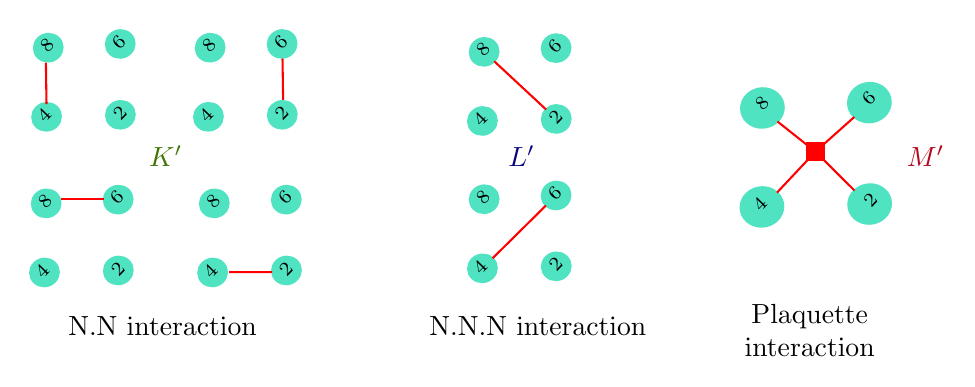
\begin{tikzpicture}[x=0.75pt,y=0.75pt,yscale=-1,xscale=1]
%uncomment if require: \path (0,574); %set diagram left start at 0, and has height of 574

%Shape: Ellipse [id:dp3297464652440131] 
\draw  [color={rgb, 255:red, 80; green, 227; blue, 194 }  ,draw opacity=1 ][fill={rgb, 255:red, 80; green, 227; blue, 194 }  ,fill opacity=1 ] (50.96,57.6) .. controls (48.26,55.08) and (48.25,50.88) .. (50.94,48.22) .. controls (53.64,45.55) and (58.02,45.43) .. (60.73,47.95) .. controls (63.43,50.47) and (63.44,54.67) .. (60.74,57.34) .. controls (58.05,60) and (53.67,60.12) .. (50.96,57.6) -- cycle ;
%Shape: Ellipse [id:dp7171372316725388] 
\draw  [color={rgb, 255:red, 80; green, 227; blue, 194 }  ,draw opacity=1 ][fill={rgb, 255:red, 80; green, 227; blue, 194 }  ,fill opacity=1 ] (50.14,90.9) .. controls (47.44,88.38) and (47.43,84.18) .. (50.12,81.52) .. controls (52.82,78.85) and (57.2,78.73) .. (59.91,81.25) .. controls (62.61,83.77) and (62.62,87.97) .. (59.92,90.64) .. controls (57.23,93.3) and (52.85,93.42) .. (50.14,90.9) -- cycle ;
%Shape: Ellipse [id:dp9576330902293114] 
\draw  [color={rgb, 255:red, 80; green, 227; blue, 194 }  ,draw opacity=1 ][fill={rgb, 255:red, 80; green, 227; blue, 194 }  ,fill opacity=1 ] (85.64,55.8) .. controls (82.94,53.29) and (82.93,49.08) .. (85.62,46.42) .. controls (88.32,43.75) and (92.7,43.63) .. (95.4,46.15) .. controls (98.11,48.67) and (98.12,52.87) .. (95.42,55.54) .. controls (92.73,58.2) and (88.35,58.32) .. (85.64,55.8) -- cycle ;
%Shape: Ellipse [id:dp2585431908339558] 
\draw  [color={rgb, 255:red, 80; green, 227; blue, 194 }  ,draw opacity=1 ][fill={rgb, 255:red, 80; green, 227; blue, 194 }  ,fill opacity=1 ] (85.71,89.94) .. controls (83.01,87.42) and (83,83.21) .. (85.69,80.55) .. controls (88.39,77.88) and (92.77,77.76) .. (95.48,80.28) .. controls (98.18,82.8) and (98.19,87) .. (95.5,89.67) .. controls (92.8,92.33) and (88.42,92.45) .. (85.71,89.94) -- cycle ;
%Shape: Ellipse [id:dp7494347016825376] 
\draw  [color={rgb, 255:red, 80; green, 227; blue, 194 }  ,draw opacity=1 ][fill={rgb, 255:red, 80; green, 227; blue, 194 }  ,fill opacity=1 ] (49.96,132.6) .. controls (47.26,130.08) and (47.25,125.88) .. (49.94,123.22) .. controls (52.64,120.55) and (57.02,120.43) .. (59.73,122.95) .. controls (62.43,125.47) and (62.44,129.67) .. (59.74,132.34) .. controls (57.05,135) and (52.67,135.12) .. (49.96,132.6) -- cycle ;
%Shape: Ellipse [id:dp08586742046422768] 
\draw  [color={rgb, 255:red, 80; green, 227; blue, 194 }  ,draw opacity=1 ][fill={rgb, 255:red, 80; green, 227; blue, 194 }  ,fill opacity=1 ] (49.14,165.9) .. controls (46.44,163.38) and (46.43,159.18) .. (49.12,156.52) .. controls (51.82,153.85) and (56.2,153.73) .. (58.91,156.25) .. controls (61.61,158.77) and (61.62,162.97) .. (58.92,165.64) .. controls (56.23,168.3) and (51.85,168.42) .. (49.14,165.9) -- cycle ;
%Shape: Ellipse [id:dp2727114151571697] 
\draw  [color={rgb, 255:red, 80; green, 227; blue, 194 }  ,draw opacity=1 ][fill={rgb, 255:red, 80; green, 227; blue, 194 }  ,fill opacity=1 ] (84.64,130.8) .. controls (81.94,128.29) and (81.93,124.08) .. (84.62,121.42) .. controls (87.32,118.75) and (91.7,118.63) .. (94.4,121.15) .. controls (97.11,123.67) and (97.12,127.87) .. (94.42,130.54) .. controls (91.73,133.2) and (87.35,133.32) .. (84.64,130.8) -- cycle ;
%Shape: Ellipse [id:dp088244480226214] 
\draw  [color={rgb, 255:red, 80; green, 227; blue, 194 }  ,draw opacity=1 ][fill={rgb, 255:red, 80; green, 227; blue, 194 }  ,fill opacity=1 ] (84.71,164.94) .. controls (82.01,162.42) and (82,158.21) .. (84.69,155.55) .. controls (87.39,152.88) and (91.77,152.76) .. (94.48,155.28) .. controls (97.18,157.8) and (97.19,162) .. (94.5,164.67) .. controls (91.8,167.33) and (87.42,167.45) .. (84.71,164.94) -- cycle ;
%Shape: Ellipse [id:dp40645145406498284] 
\draw  [color={rgb, 255:red, 80; green, 227; blue, 194 }  ,draw opacity=1 ][fill={rgb, 255:red, 80; green, 227; blue, 194 }  ,fill opacity=1 ] (128.96,57.6) .. controls (126.26,55.08) and (126.25,50.88) .. (128.94,48.22) .. controls (131.64,45.55) and (136.02,45.43) .. (138.73,47.95) .. controls (141.43,50.47) and (141.44,54.67) .. (138.74,57.34) .. controls (136.05,60) and (131.67,60.12) .. (128.96,57.6) -- cycle ;
%Shape: Ellipse [id:dp13015019196252697] 
\draw  [color={rgb, 255:red, 80; green, 227; blue, 194 }  ,draw opacity=1 ][fill={rgb, 255:red, 80; green, 227; blue, 194 }  ,fill opacity=1 ] (128.14,90.9) .. controls (125.44,88.38) and (125.43,84.18) .. (128.12,81.52) .. controls (130.82,78.85) and (135.2,78.73) .. (137.91,81.25) .. controls (140.61,83.77) and (140.62,87.97) .. (137.92,90.64) .. controls (135.23,93.3) and (130.85,93.42) .. (128.14,90.9) -- cycle ;
%Shape: Ellipse [id:dp04472277592997875] 
\draw  [color={rgb, 255:red, 80; green, 227; blue, 194 }  ,draw opacity=1 ][fill={rgb, 255:red, 80; green, 227; blue, 194 }  ,fill opacity=1 ] (163.64,55.8) .. controls (160.94,53.29) and (160.93,49.08) .. (163.62,46.42) .. controls (166.32,43.75) and (170.7,43.63) .. (173.4,46.15) .. controls (176.11,48.67) and (176.12,52.87) .. (173.42,55.54) .. controls (170.73,58.2) and (166.35,58.32) .. (163.64,55.8) -- cycle ;
%Shape: Ellipse [id:dp35910086528484764] 
\draw  [color={rgb, 255:red, 80; green, 227; blue, 194 }  ,draw opacity=1 ][fill={rgb, 255:red, 80; green, 227; blue, 194 }  ,fill opacity=1 ] (163.71,89.94) .. controls (161.01,87.42) and (161,83.21) .. (163.69,80.55) .. controls (166.39,77.88) and (170.77,77.76) .. (173.48,80.28) .. controls (176.18,82.8) and (176.19,87) .. (173.5,89.67) .. controls (170.8,92.33) and (166.42,92.45) .. (163.71,89.94) -- cycle ;
%Shape: Ellipse [id:dp3909568617302668] 
\draw  [color={rgb, 255:red, 80; green, 227; blue, 194 }  ,draw opacity=1 ][fill={rgb, 255:red, 80; green, 227; blue, 194 }  ,fill opacity=1 ] (130.96,132.6) .. controls (128.26,130.08) and (128.25,125.88) .. (130.94,123.22) .. controls (133.64,120.55) and (138.02,120.43) .. (140.73,122.95) .. controls (143.43,125.47) and (143.44,129.67) .. (140.74,132.34) .. controls (138.05,135) and (133.67,135.12) .. (130.96,132.6) -- cycle ;
%Shape: Ellipse [id:dp820759586276344] 
\draw  [color={rgb, 255:red, 80; green, 227; blue, 194 }  ,draw opacity=1 ][fill={rgb, 255:red, 80; green, 227; blue, 194 }  ,fill opacity=1 ] (130.14,165.9) .. controls (127.44,163.38) and (127.43,159.18) .. (130.12,156.52) .. controls (132.82,153.85) and (137.2,153.73) .. (139.91,156.25) .. controls (142.61,158.77) and (142.62,162.97) .. (139.92,165.64) .. controls (137.23,168.3) and (132.85,168.42) .. (130.14,165.9) -- cycle ;
%Shape: Ellipse [id:dp34946155437387993] 
\draw  [color={rgb, 255:red, 80; green, 227; blue, 194 }  ,draw opacity=1 ][fill={rgb, 255:red, 80; green, 227; blue, 194 }  ,fill opacity=1 ] (165.64,130.8) .. controls (162.94,128.29) and (162.93,124.08) .. (165.62,121.42) .. controls (168.32,118.75) and (172.7,118.63) .. (175.4,121.15) .. controls (178.11,123.67) and (178.12,127.87) .. (175.42,130.54) .. controls (172.73,133.2) and (168.35,133.32) .. (165.64,130.8) -- cycle ;
%Shape: Ellipse [id:dp9652167022277574] 
\draw  [color={rgb, 255:red, 80; green, 227; blue, 194 }  ,draw opacity=1 ][fill={rgb, 255:red, 80; green, 227; blue, 194 }  ,fill opacity=1 ] (165.71,164.94) .. controls (163.01,162.42) and (163,158.21) .. (165.69,155.55) .. controls (168.39,152.88) and (172.77,152.76) .. (175.48,155.28) .. controls (178.18,157.8) and (178.19,162) .. (175.5,164.67) .. controls (172.8,167.33) and (168.42,167.45) .. (165.71,164.94) -- cycle ;
%Shape: Ellipse [id:dp5629980341205785] 
\draw  [color={rgb, 255:red, 80; green, 227; blue, 194 }  ,draw opacity=1 ][fill={rgb, 255:red, 80; green, 227; blue, 194 }  ,fill opacity=1 ] (260.96,59.6) .. controls (258.26,57.08) and (258.25,52.88) .. (260.94,50.22) .. controls (263.64,47.55) and (268.02,47.43) .. (270.73,49.95) .. controls (273.43,52.47) and (273.44,56.67) .. (270.74,59.34) .. controls (268.05,62) and (263.67,62.12) .. (260.96,59.6) -- cycle ;
%Shape: Ellipse [id:dp663757350138148] 
\draw  [color={rgb, 255:red, 80; green, 227; blue, 194 }  ,draw opacity=1 ][fill={rgb, 255:red, 80; green, 227; blue, 194 }  ,fill opacity=1 ] (260.14,92.9) .. controls (257.44,90.38) and (257.43,86.18) .. (260.12,83.52) .. controls (262.82,80.85) and (267.2,80.73) .. (269.91,83.25) .. controls (272.61,85.77) and (272.62,89.97) .. (269.92,92.64) .. controls (267.23,95.3) and (262.85,95.42) .. (260.14,92.9) -- cycle ;
%Shape: Ellipse [id:dp9120008419253309] 
\draw  [color={rgb, 255:red, 80; green, 227; blue, 194 }  ,draw opacity=1 ][fill={rgb, 255:red, 80; green, 227; blue, 194 }  ,fill opacity=1 ] (295.64,57.8) .. controls (292.94,55.29) and (292.93,51.08) .. (295.62,48.42) .. controls (298.32,45.75) and (302.7,45.63) .. (305.4,48.15) .. controls (308.11,50.67) and (308.12,54.87) .. (305.42,57.54) .. controls (302.73,60.2) and (298.35,60.32) .. (295.64,57.8) -- cycle ;
%Shape: Ellipse [id:dp9542659694204088] 
\draw  [color={rgb, 255:red, 80; green, 227; blue, 194 }  ,draw opacity=1 ][fill={rgb, 255:red, 80; green, 227; blue, 194 }  ,fill opacity=1 ] (295.71,91.94) .. controls (293.01,89.42) and (293,85.21) .. (295.69,82.55) .. controls (298.39,79.88) and (302.77,79.76) .. (305.48,82.28) .. controls (308.18,84.8) and (308.19,89) .. (305.5,91.67) .. controls (302.8,94.33) and (298.42,94.45) .. (295.71,91.94) -- cycle ;
%Shape: Ellipse [id:dp6106279760925897] 
\draw  [color={rgb, 255:red, 80; green, 227; blue, 194 }  ,draw opacity=1 ][fill={rgb, 255:red, 80; green, 227; blue, 194 }  ,fill opacity=1 ] (260.96,130.6) .. controls (258.26,128.08) and (258.25,123.88) .. (260.94,121.22) .. controls (263.64,118.55) and (268.02,118.43) .. (270.73,120.95) .. controls (273.43,123.47) and (273.44,127.67) .. (270.74,130.34) .. controls (268.05,133) and (263.67,133.12) .. (260.96,130.6) -- cycle ;
%Shape: Ellipse [id:dp3031437328186797] 
\draw  [color={rgb, 255:red, 80; green, 227; blue, 194 }  ,draw opacity=1 ][fill={rgb, 255:red, 80; green, 227; blue, 194 }  ,fill opacity=1 ] (260.14,163.9) .. controls (257.44,161.38) and (257.43,157.18) .. (260.12,154.52) .. controls (262.82,151.85) and (267.2,151.73) .. (269.91,154.25) .. controls (272.61,156.77) and (272.62,160.97) .. (269.92,163.64) .. controls (267.23,166.3) and (262.85,166.42) .. (260.14,163.9) -- cycle ;
%Shape: Ellipse [id:dp4050857241629019] 
\draw  [color={rgb, 255:red, 80; green, 227; blue, 194 }  ,draw opacity=1 ][fill={rgb, 255:red, 80; green, 227; blue, 194 }  ,fill opacity=1 ] (295.64,128.8) .. controls (292.94,126.29) and (292.93,122.08) .. (295.62,119.42) .. controls (298.32,116.75) and (302.7,116.63) .. (305.4,119.15) .. controls (308.11,121.67) and (308.12,125.87) .. (305.42,128.54) .. controls (302.73,131.2) and (298.35,131.32) .. (295.64,128.8) -- cycle ;
%Shape: Ellipse [id:dp5486208963659012] 
\draw  [color={rgb, 255:red, 80; green, 227; blue, 194 }  ,draw opacity=1 ][fill={rgb, 255:red, 80; green, 227; blue, 194 }  ,fill opacity=1 ] (295.71,162.94) .. controls (293.01,160.42) and (293,156.21) .. (295.69,153.55) .. controls (298.39,150.88) and (302.77,150.76) .. (305.48,153.28) .. controls (308.18,155.8) and (308.19,160) .. (305.5,162.67) .. controls (302.8,165.33) and (298.42,165.45) .. (295.71,162.94) -- cycle ;
%Shape: Ellipse [id:dp6718099050301578] 
\draw  [color={rgb, 255:red, 80; green, 227; blue, 194 }  ,draw opacity=1 ][fill={rgb, 255:red, 80; green, 227; blue, 194 }  ,fill opacity=1 ] (392.66,88.72) .. controls (388.64,85.12) and (388.63,79.1) .. (392.63,75.28) .. controls (396.64,71.47) and (403.15,71.3) .. (407.18,74.9) .. controls (411.2,78.51) and (411.21,84.52) .. (407.2,88.34) .. controls (403.19,92.16) and (396.68,92.33) .. (392.66,88.72) -- cycle ;
%Shape: Ellipse [id:dp03605076666804796] 
\draw  [color={rgb, 255:red, 80; green, 227; blue, 194 }  ,draw opacity=1 ][fill={rgb, 255:red, 80; green, 227; blue, 194 }  ,fill opacity=1 ] (392.44,136.4) .. controls (388.42,132.79) and (388.41,126.78) .. (392.42,122.96) .. controls (396.43,119.14) and (402.94,118.97) .. (406.96,122.58) .. controls (410.98,126.18) and (410.99,132.2) .. (406.98,136.02) .. controls (402.98,139.83) and (396.47,140) .. (392.44,136.4) -- cycle ;
%Shape: Ellipse [id:dp42705804901053] 
\draw  [color={rgb, 255:red, 80; green, 227; blue, 194 }  ,draw opacity=1 ][fill={rgb, 255:red, 80; green, 227; blue, 194 }  ,fill opacity=1 ] (444.21,86.15) .. controls (440.19,82.54) and (440.18,76.53) .. (444.19,72.71) .. controls (448.2,68.9) and (454.71,68.73) .. (458.73,72.33) .. controls (462.75,75.94) and (462.76,81.95) .. (458.75,85.77) .. controls (454.75,89.58) and (448.24,89.75) .. (444.21,86.15) -- cycle ;
%Shape: Ellipse [id:dp13485884930115344] 
\draw  [color={rgb, 255:red, 80; green, 227; blue, 194 }  ,draw opacity=1 ][fill={rgb, 255:red, 80; green, 227; blue, 194 }  ,fill opacity=1 ] (444.32,135.01) .. controls (440.3,131.41) and (440.29,125.39) .. (444.29,121.58) .. controls (448.3,117.76) and (454.81,117.59) .. (458.84,121.19) .. controls (462.86,124.8) and (462.87,130.82) .. (458.86,134.63) .. controls (454.85,138.45) and (448.34,138.62) .. (444.32,135.01) -- cycle ;
%Straight Lines [id:da30065043590674634] 
\draw [color={rgb, 255:red, 255; green, 0; blue, 0 }  ,draw opacity=1 ]   (54.71,60) -- (55,79.93) ;
%Straight Lines [id:da7965055761102636] 
\draw [color={rgb, 255:red, 255; green, 0; blue, 0 }  ,draw opacity=1 ]   (168.71,58) -- (169,77.93) ;
%Straight Lines [id:da9730162601844693] 
\draw [color={rgb, 255:red, 255; green, 0; blue, 0 }  ,draw opacity=1 ]   (163.71,160.94) -- (143,160.93) ;
%Straight Lines [id:da021942434453994575] 
\draw [color={rgb, 255:red, 255; green, 0; blue, 0 }  ,draw opacity=1 ]   (82.64,125.8) -- (61.93,125.8) ;
%Straight Lines [id:da8772824595252458] 
\draw [color={rgb, 255:red, 255; green, 0; blue, 0 }  ,draw opacity=1 ]   (295.69,82.55) -- (270.74,59.34) ;
%Straight Lines [id:da7264690434415212] 
\draw [color={rgb, 255:red, 255; green, 0; blue, 0 }  ,draw opacity=1 ]   (295.64,128.8) -- (269.91,154.25) ;
%Straight Lines [id:da6019995240575259] 
\draw [color={rgb, 255:red, 255; green, 0; blue, 0 }  ,draw opacity=1 ]   (425.46,102.87) -- (407.2,88.34) ;
%Shape: Square [id:dp407517584926799] 
\draw  [color={rgb, 255:red, 255; green, 0; blue, 0 }  ,draw opacity=1 ][fill={rgb, 255:red, 255; green, 0; blue, 0 }  ,fill opacity=1 ] (421.46,98.87) -- (429.46,98.87) -- (429.46,106.87) -- (421.46,106.87) -- cycle ;
%Straight Lines [id:da9902573103931569] 
\draw [color={rgb, 255:red, 255; green, 0; blue, 0 }  ,draw opacity=1 ]   (425.46,102.87) -- (406.96,122.58) ;
%Straight Lines [id:da6530425560088687] 
\draw [color={rgb, 255:red, 255; green, 0; blue, 0 }  ,draw opacity=1 ]   (425.46,102.87) -- (444.29,121.58) ;
%Straight Lines [id:da49038104114151093] 
\draw [color={rgb, 255:red, 255; green, 0; blue, 0 }  ,draw opacity=1 ]   (444.21,86.15) -- (425.46,102.87) ;

% Text Node
\draw (84.26,84.15) node [anchor=north west][inner sep=0.75pt]  [font=\scriptsize,rotate=-314.13]  {$2$};
% Text Node
\draw (47.83,85.28) node [anchor=north west][inner sep=0.75pt]  [font=\scriptsize,rotate=-314.13]  {$4$};
% Text Node
\draw (83.72,49.79) node [anchor=north west][inner sep=0.75pt]  [font=\scriptsize,rotate=-314.13]  {$6$};
% Text Node
\draw (49.15,51.48) node [anchor=north west][inner sep=0.75pt]  [font=\scriptsize,rotate=-314.13]  {$8$};
% Text Node
\draw (83.26,159.15) node [anchor=north west][inner sep=0.75pt]  [font=\scriptsize,rotate=-314.13]  {$2$};
% Text Node
\draw (46.83,160.28) node [anchor=north west][inner sep=0.75pt]  [font=\scriptsize,rotate=-314.13]  {$4$};
% Text Node
\draw (82.72,124.79) node [anchor=north west][inner sep=0.75pt]  [font=\scriptsize,rotate=-314.13]  {$6$};
% Text Node
\draw (48.15,126.48) node [anchor=north west][inner sep=0.75pt]  [font=\scriptsize,rotate=-314.13]  {$8$};
% Text Node
\draw (162.26,84.15) node [anchor=north west][inner sep=0.75pt]  [font=\scriptsize,rotate=-314.13]  {$2$};
% Text Node
\draw (125.83,85.28) node [anchor=north west][inner sep=0.75pt]  [font=\scriptsize,rotate=-314.13]  {$4$};
% Text Node
\draw (161.72,49.79) node [anchor=north west][inner sep=0.75pt]  [font=\scriptsize,rotate=-314.13]  {$6$};
% Text Node
\draw (127.15,51.48) node [anchor=north west][inner sep=0.75pt]  [font=\scriptsize,rotate=-314.13]  {$8$};
% Text Node
\draw (164.26,159.15) node [anchor=north west][inner sep=0.75pt]  [font=\scriptsize,rotate=-314.13]  {$2$};
% Text Node
\draw (127.83,160.28) node [anchor=north west][inner sep=0.75pt]  [font=\scriptsize,rotate=-314.13]  {$4$};
% Text Node
\draw (163.72,124.79) node [anchor=north west][inner sep=0.75pt]  [font=\scriptsize,rotate=-314.13]  {$6$};
% Text Node
\draw (129.15,126.48) node [anchor=north west][inner sep=0.75pt]  [font=\scriptsize,rotate=-314.13]  {$8$};
% Text Node
\draw (294.26,86.15) node [anchor=north west][inner sep=0.75pt]  [font=\scriptsize,rotate=-314.13]  {$2$};
% Text Node
\draw (257.83,87.28) node [anchor=north west][inner sep=0.75pt]  [font=\scriptsize,rotate=-314.13]  {$4$};
% Text Node
\draw (293.72,51.79) node [anchor=north west][inner sep=0.75pt]  [font=\scriptsize,rotate=-314.13]  {$6$};
% Text Node
\draw (259.15,53.48) node [anchor=north west][inner sep=0.75pt]  [font=\scriptsize,rotate=-314.13]  {$8$};
% Text Node
\draw (294.26,157.15) node [anchor=north west][inner sep=0.75pt]  [font=\scriptsize,rotate=-314.13]  {$2$};
% Text Node
\draw (257.83,158.28) node [anchor=north west][inner sep=0.75pt]  [font=\scriptsize,rotate=-314.13]  {$4$};
% Text Node
\draw (293.72,122.79) node [anchor=north west][inner sep=0.75pt]  [font=\scriptsize,rotate=-314.13]  {$6$};
% Text Node
\draw (259.15,124.48) node [anchor=north west][inner sep=0.75pt]  [font=\scriptsize,rotate=-314.13]  {$8$};
% Text Node
\draw (445.81,126.26) node [anchor=north west][inner sep=0.75pt]  [font=\scriptsize,rotate=-314.13]  {$2$};
% Text Node
\draw (392.65,127.87) node [anchor=north west][inner sep=0.75pt]  [font=\scriptsize,rotate=-314.13]  {$4$};
% Text Node
\draw (445,77.07) node [anchor=north west][inner sep=0.75pt]  [font=\scriptsize,rotate=-314.13]  {$6$};
% Text Node
\draw (393.61,79.48) node [anchor=north west][inner sep=0.75pt]  [font=\scriptsize,rotate=-314.13]  {$8$};
% Text Node
\draw (64,181) node [anchor=north west][inner sep=0.75pt]   [align=left] {N.N interaction};
% Text Node
\draw (238,181) node [anchor=north west][inner sep=0.75pt]   [align=left] {N.N.N interaction};
% Text Node
\draw (386,175) node [anchor=north west][inner sep=0.75pt]   [align=left] {\begin{minipage}[lt]{52.81pt}\setlength\topsep{0pt}
\begin{center}
Plaquette \\interaction
\end{center}

\end{minipage}};
% Text Node
\draw (103,98.4) node [anchor=north west][inner sep=0.75pt]  [color={rgb, 255:red, 65; green, 117; blue, 5 }  ,opacity=1 ]  {$K'$};
% Text Node
\draw (276,98.4) node [anchor=north west][inner sep=0.75pt]  [color={rgb, 255:red, 7; green, 5; blue, 129 }  ,opacity=1 ]  {$L'$};
% Text Node
\draw (468,98.4) node [anchor=north west][inner sep=0.75pt]  [color={rgb, 255:red, 182; green, 6; blue, 29 }  ,opacity=1 ]  {$M'$};


\end{tikzpicture}

    \caption{Type of interactions generated after one round of decimation.}
\end{figure}
\noindent
To make a way around this problem of not having a correspondence with the original Hamiltonian, we assume that the initial Hamiltonian was also of the same form, with all these interactions, but the corresponding couplings were $0$. So $L=M=0$ for the original system. Then we can write,
\begin{align*}
    \SZ_{N}(\qty{K,0,0}) = e^{N' K_0'}\SZ_{N'}(\qty{K',L',M'}) \implies \zeta(\qty{K,0,0}) = -\frac{1}{2}K_0' + \frac{1}{2}\zeta(\qty{K',L',M'})
\end{align*}
The number of parameters will increase after each round of decimation and the problem will become intractable unless we do what we \textit{love} to do: take weird approximations! In here, we will assume that only the nearest ($K$) and the next-nearest neighbour interactions ($L$) are important and further, that these are very small (so $\cosh(x)\approx 1 +\frac{x^2}{2}$ and $\ln \qty(1 +\frac{x^2}{2})\approx \frac{x^2}{2}$), which changes Eq. \eqref{recrel2d} to,
$$K' = 2K^2\qquad L' = K^2$$
Furthermore, let us suppose that $L\neq 0$ in the beginning. Then, considering this we would have obtained the transformations as $$K'= 2K^2 + L \qquad L'=K^2$$ 
Now, we need to find the fixed point of these transformations.
$$L^* = K^{*2}\qquad K^*=2K^{*2}+L^* = 3K^{*2}$$
This gives us two set of fixed points, $(K^*,L^*) = (0,0)$ and $(K^*,L^*) = (\sfrac{1}{3},\sfrac{1}{9})$. The first one is the trivial fixed point, corresponding to infinite temperature, while the second one is the one of our interest.\\[0.2cm]
Considering deviations from the fixed point, $K = K^*+\delta K$ and $L=L^*+\delta L$, we get:
\begin{align*}
   K^*+\delta K' \equiv  K' &= 2(K^*+\delta K)^2 + (\delta L + L^*) = \mathcolor{red}{2K^{*2}} + 4K^*\delta K +\delta L + \mathcolor{red}{L^*} = \mathcolor{red}{K^*}+4K^*\delta K+\delta L\\
   L^*+\delta L' \equiv L' &= \mathcolor{red}{K^{*2}} + 2K^* \delta K = \mathcolor{red}{L^*}+2K^* \delta K
\end{align*}
From this, we get the following in matrix form, 
\begin{equation}
    \mqty(\delta K' \\ \delta L') = \mqty( 4K^* & 1 \\ 2K^* & 0 ) \mqty(\delta K \\ \delta L)\quad \longrightarrow\quad \boxed{\mqty(\delta K' \\ \delta L') =\mqty( \sfrac{4}{3} & 1 \\ \sfrac{2}{3} & 0 ) \mqty(\delta K \\ \delta L)}
\end{equation}
Before the transformation, we have the lattice spacing as $a$ and after transformation, the lattice spacing becomes $a'= a\sqrt{2}$ which implies that $l=\sqrt{2}$. The linearised RG is thus, 
$$\mathrm{M}^{(\sqrt{2})} \equiv \mqty( \sfrac{4}{3} & 1 \\ \sfrac{2}{3} & 0 ) $$